
\documentclass[../main.tex]{subfiles}
\begin{document}
\setlength\parindent{24pt}
% 1
\section{Generation of an OFDM Waveform}

% 1.1
\subsection{Waveform Spectrum}

% 1.1.1
\subsubsection{}
{No discussion necessary.}

% 1.1.2
\subsubsection{}
{No discussion necessary.}

% 1.1.3
\subsubsection{}
{No discussion necessary.}
\newpage

% 1.1.4
\subsubsection{}
\begin{figure}[H]
   \centering
   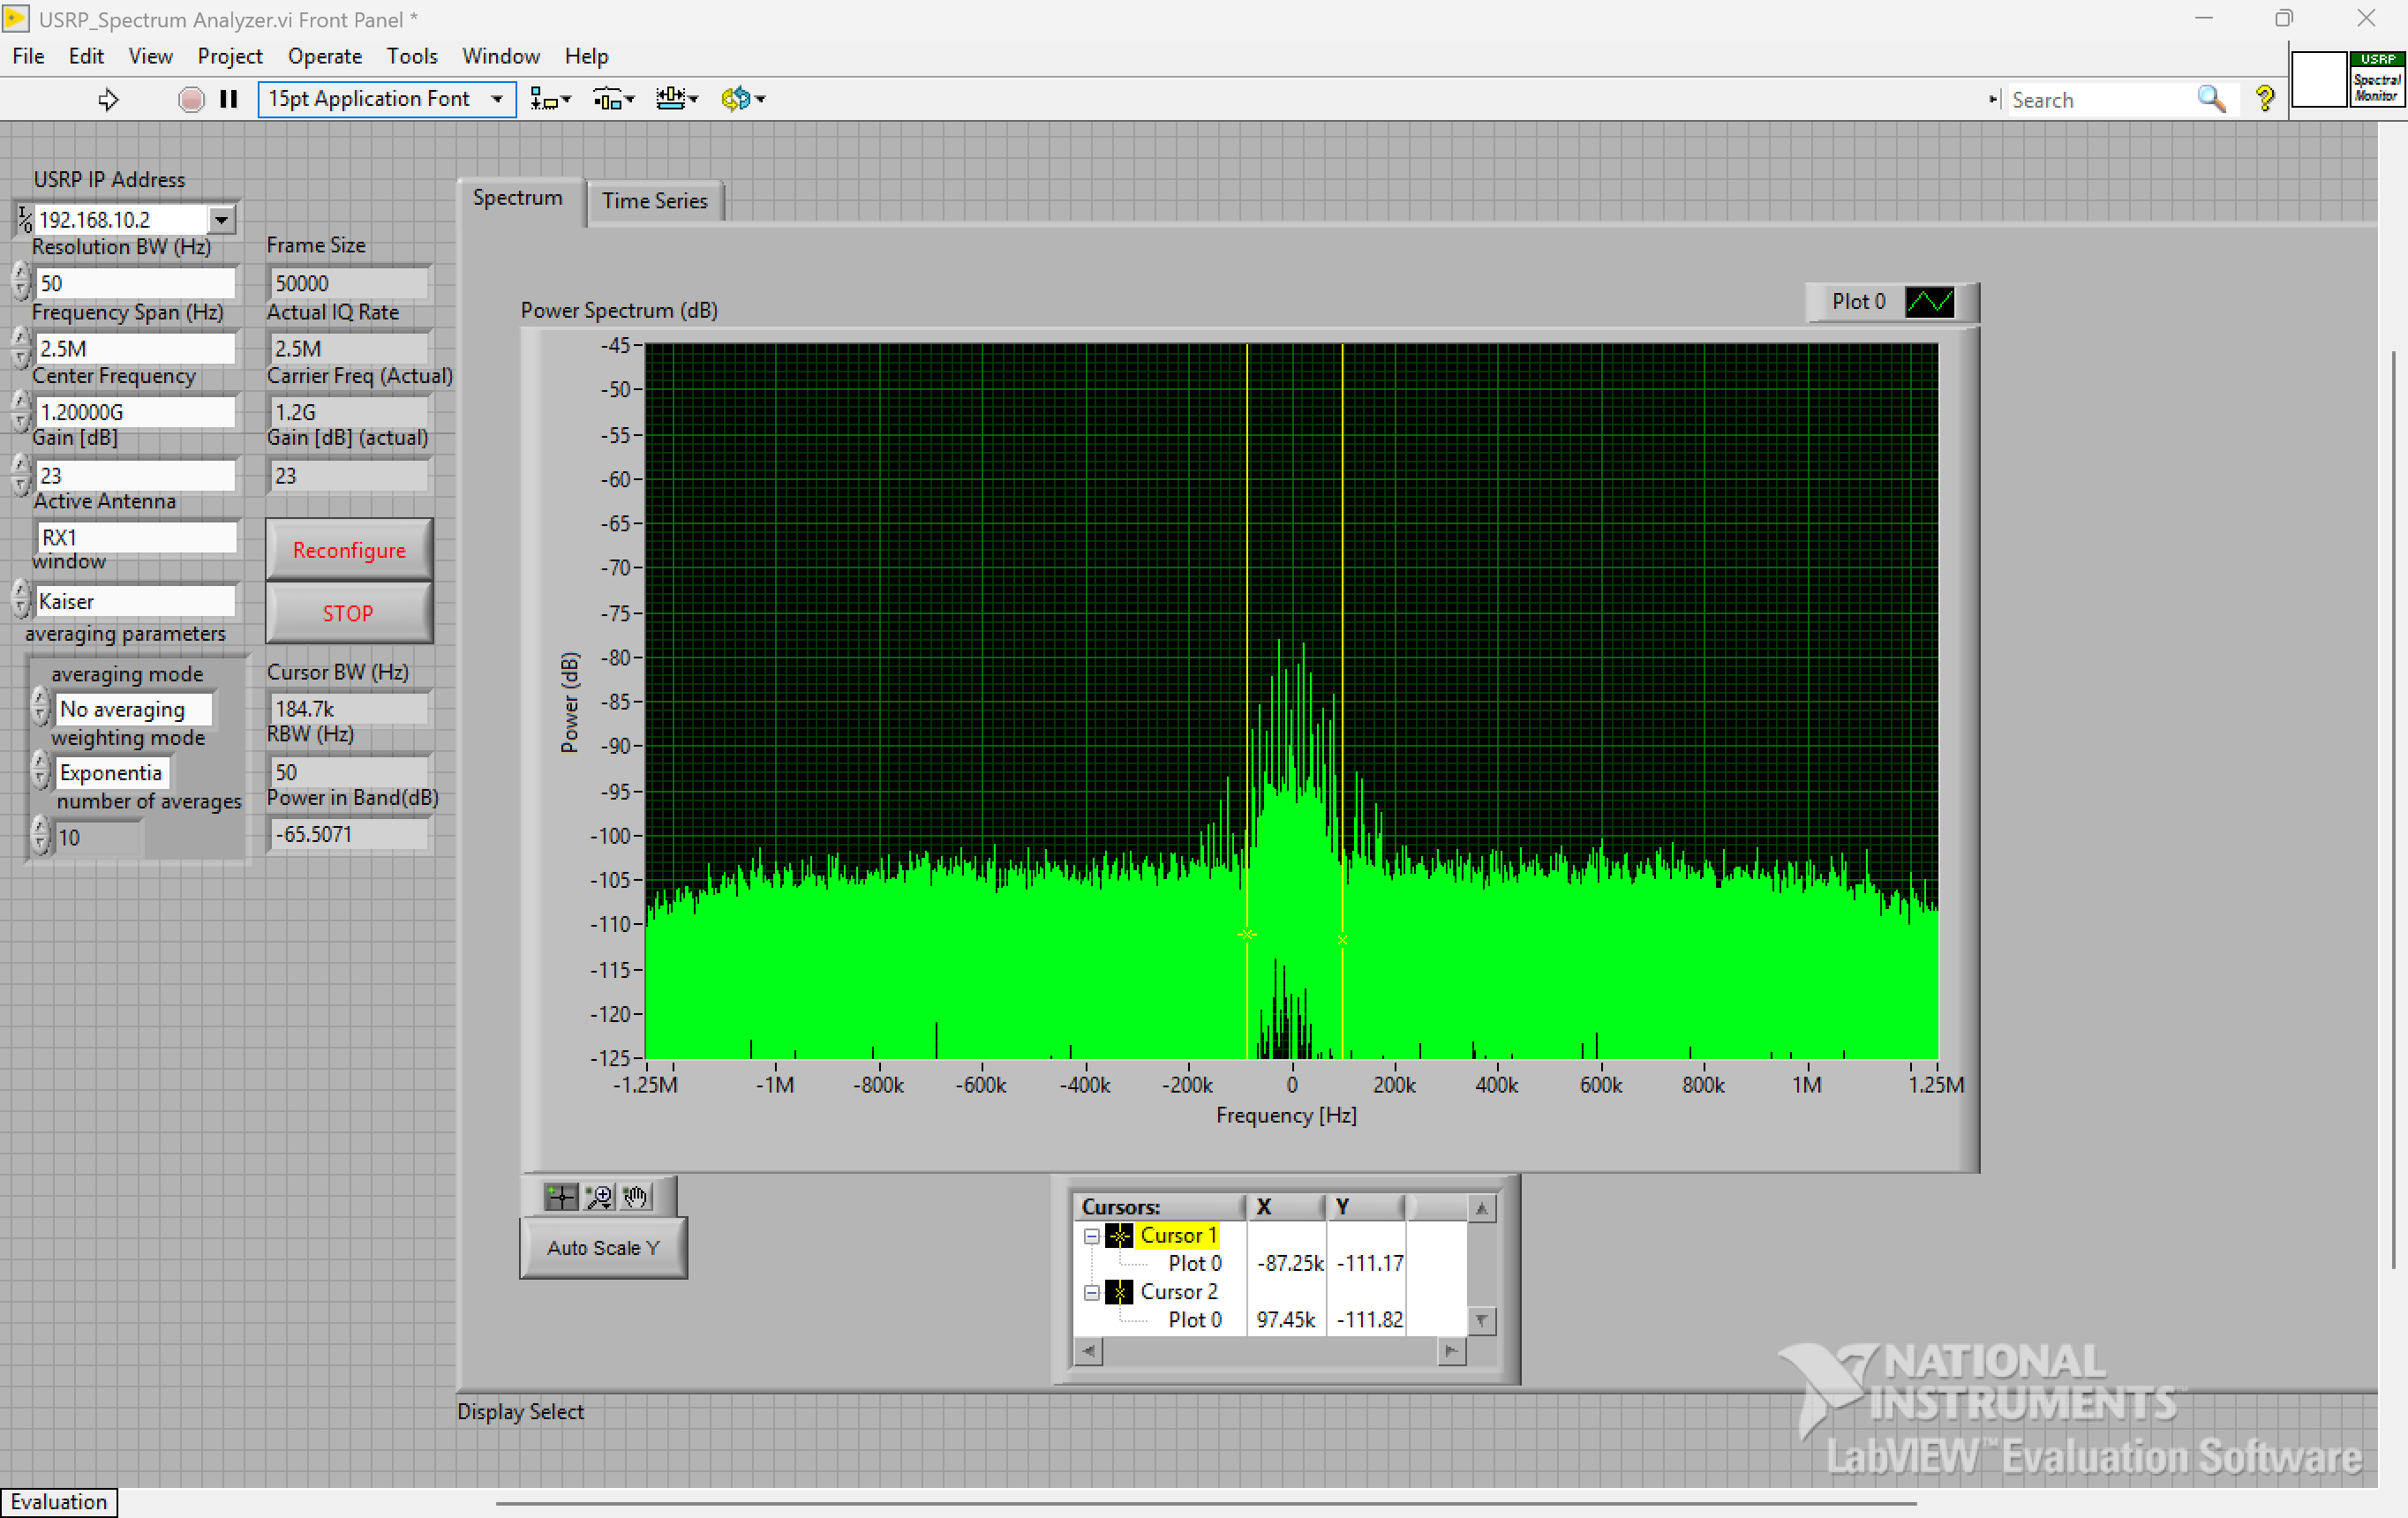
\includegraphics[width=0.7\textwidth]{../lab_ss/WES268B_Lab6_Part1-1-4_measured-null-to-null-bw_184khz.png}
   \caption{1.1.4 - Measured Null-to-Null Bandwidth, 184kHz}
\end{figure}
\par

% 1.1.5
\subsubsection{}
\begin{figure}[H]
   \centering
   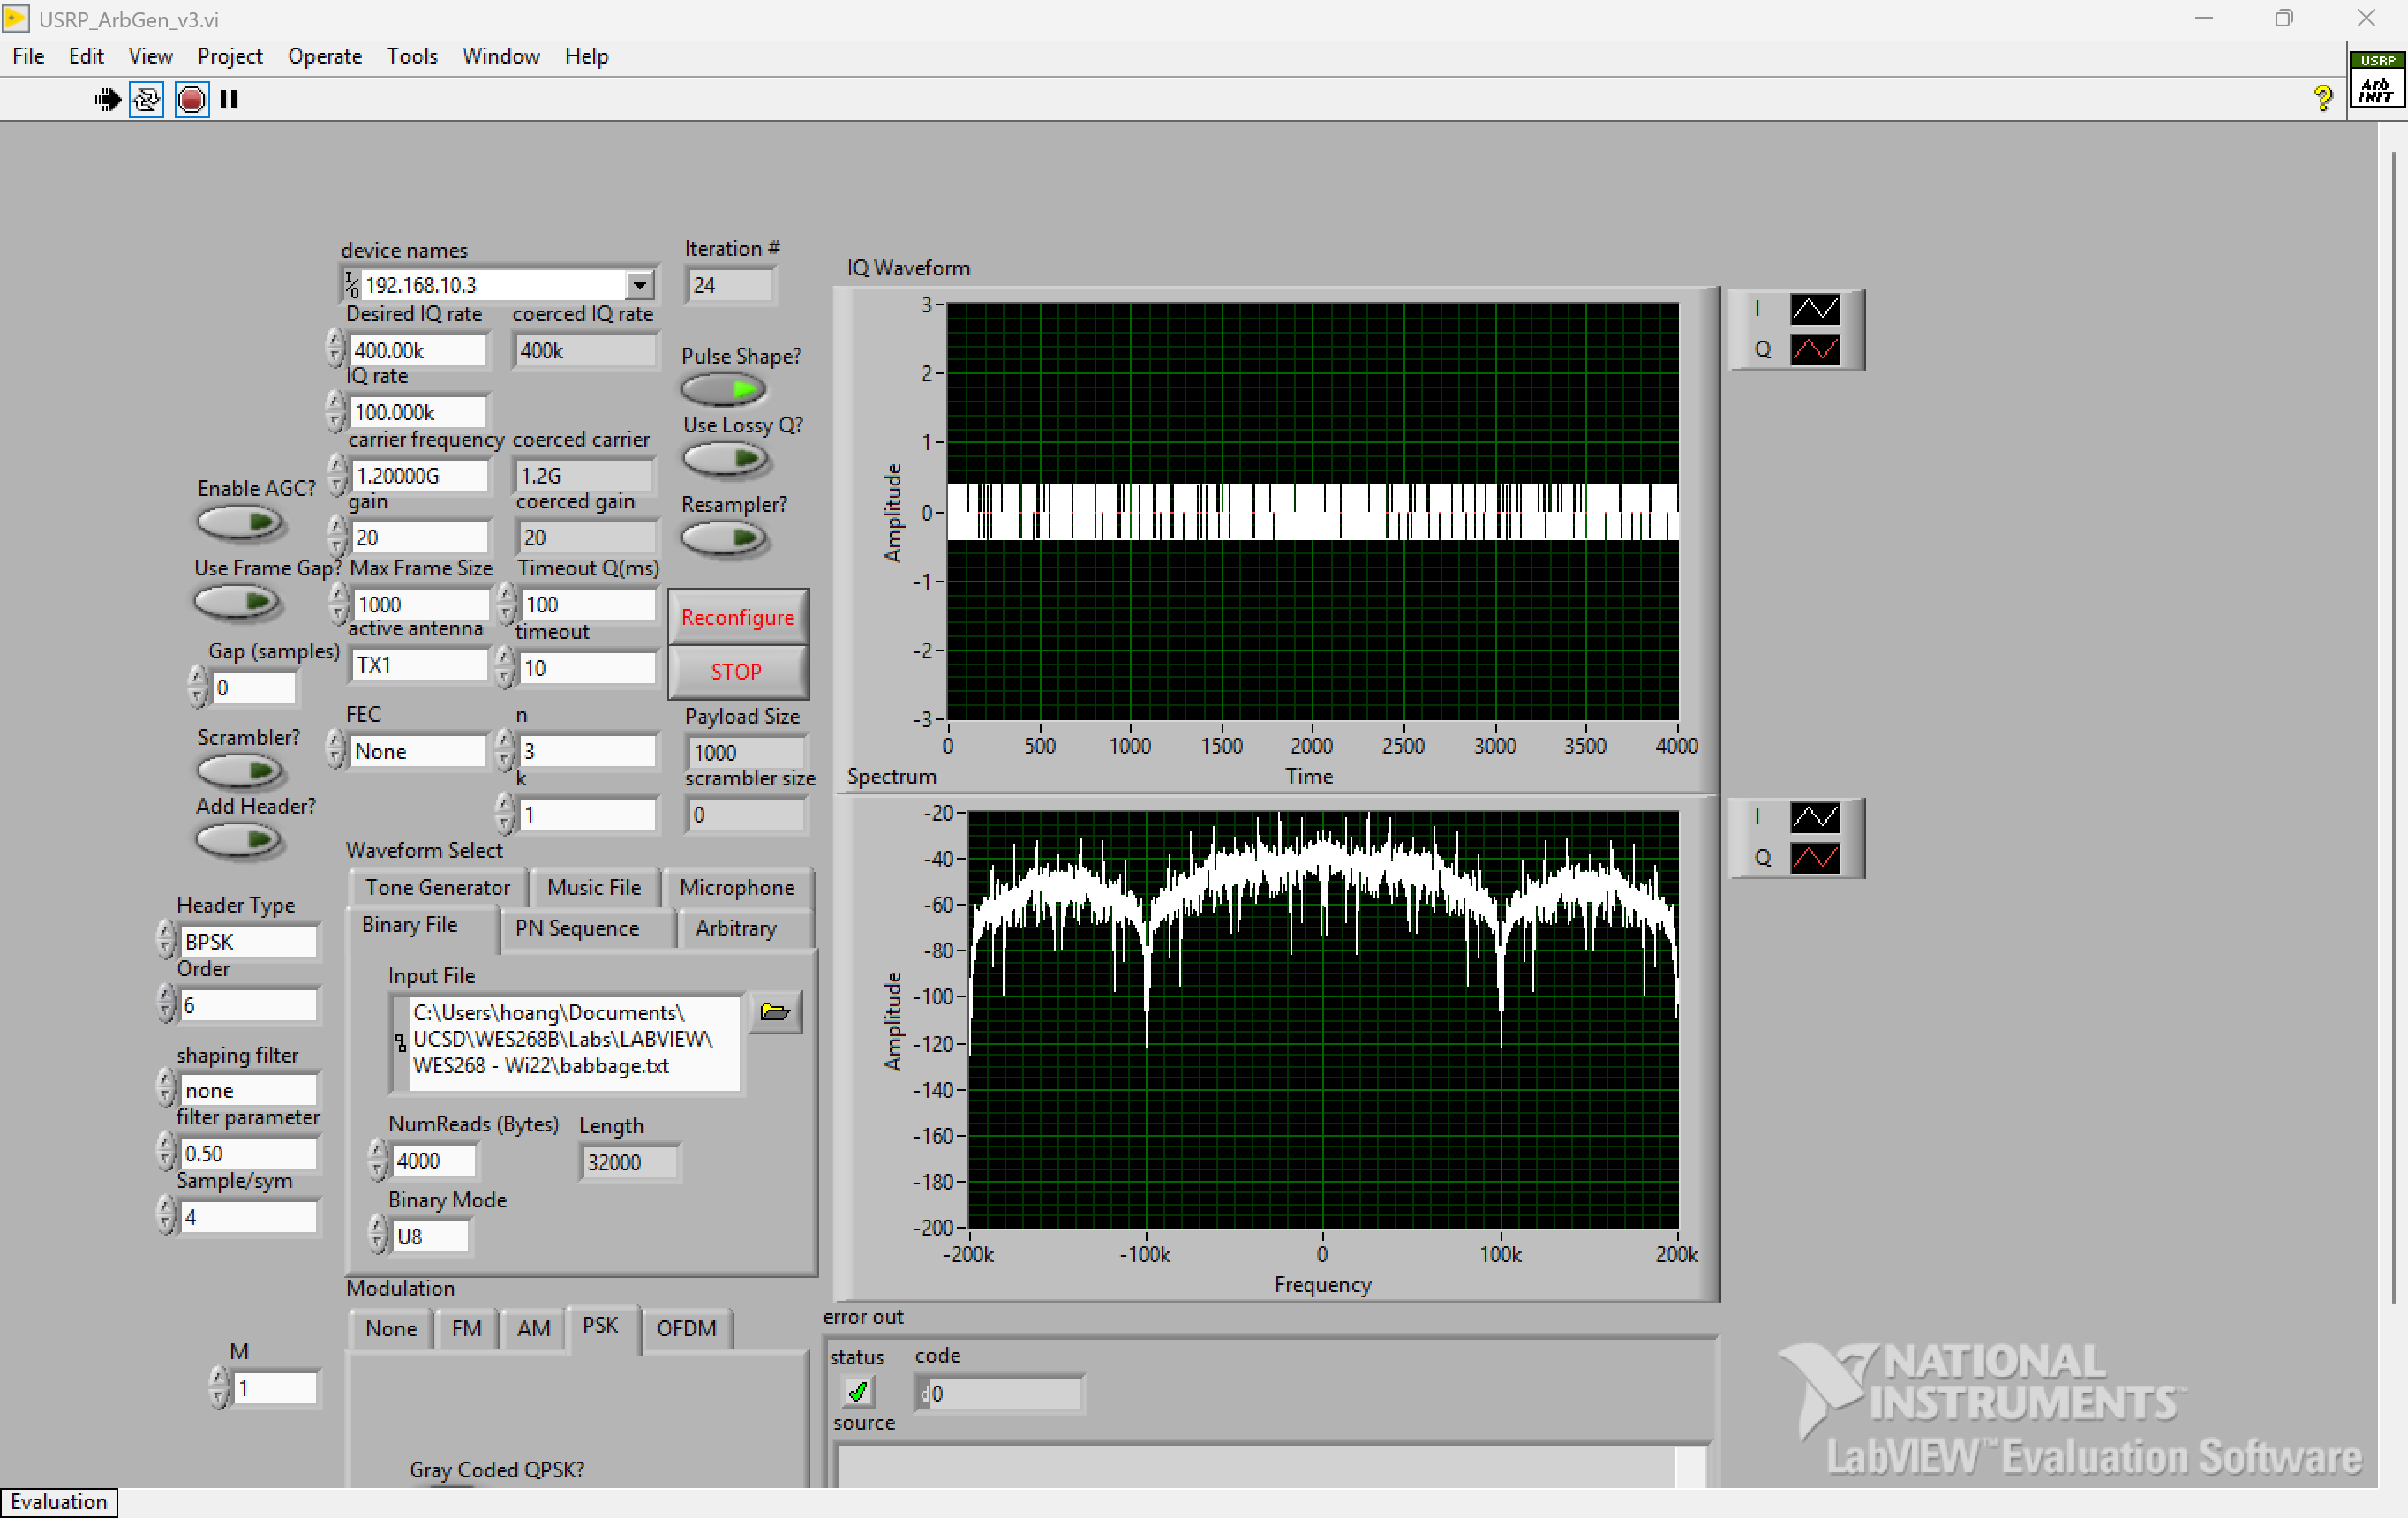
\includegraphics[width=0.7\textwidth]{../lab_ss/WES268B_Lab6_Part1-1-5_Tx.png}
   \caption{1.1.5 - Transmitted Spectrum of above signal}
\end{figure}
\par
\newpage

% 1.1.6
\subsubsection{}
\begin{figure}[H]
   \centering
   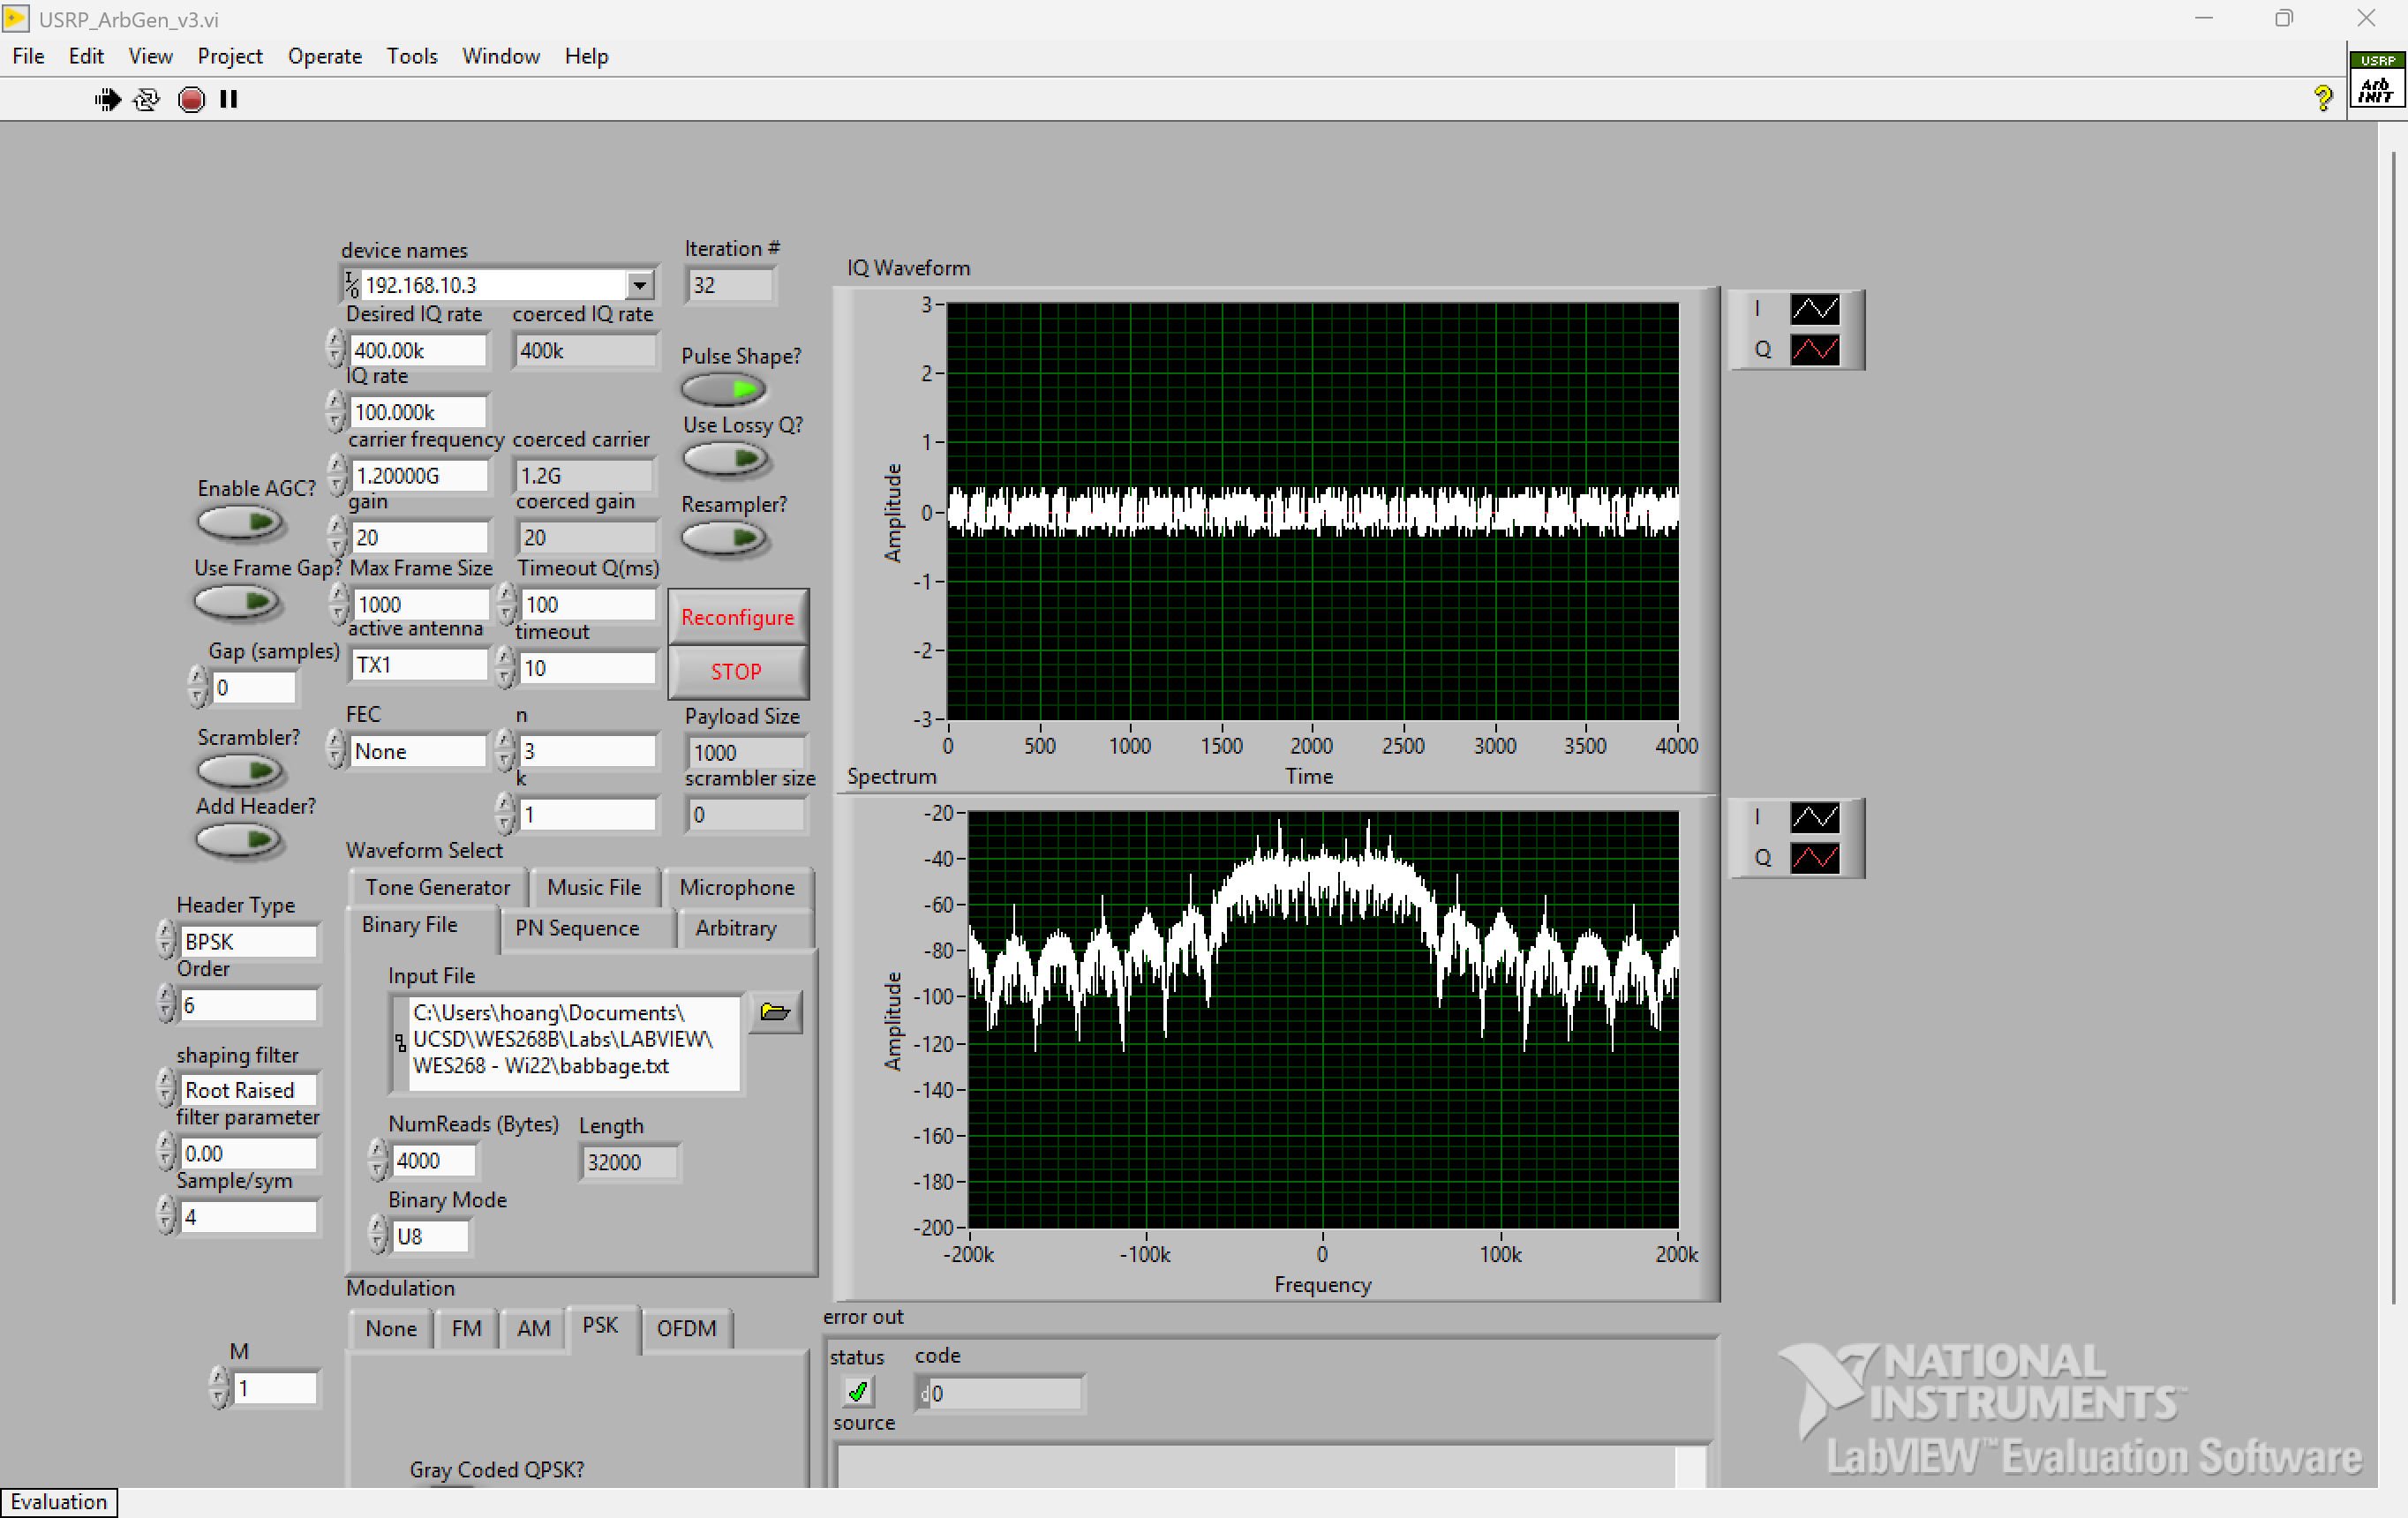
\includegraphics[width=0.7\textwidth]
   {../lab_ss/WES268B_Lab6_Part1-1-6_Tx_root-raised_filter-parameter-0.png}
   \caption{1.1.6 - TX RRC, $\beta = 0$}
\end{figure}
\par
\begin{figure}[H]
   \centering
   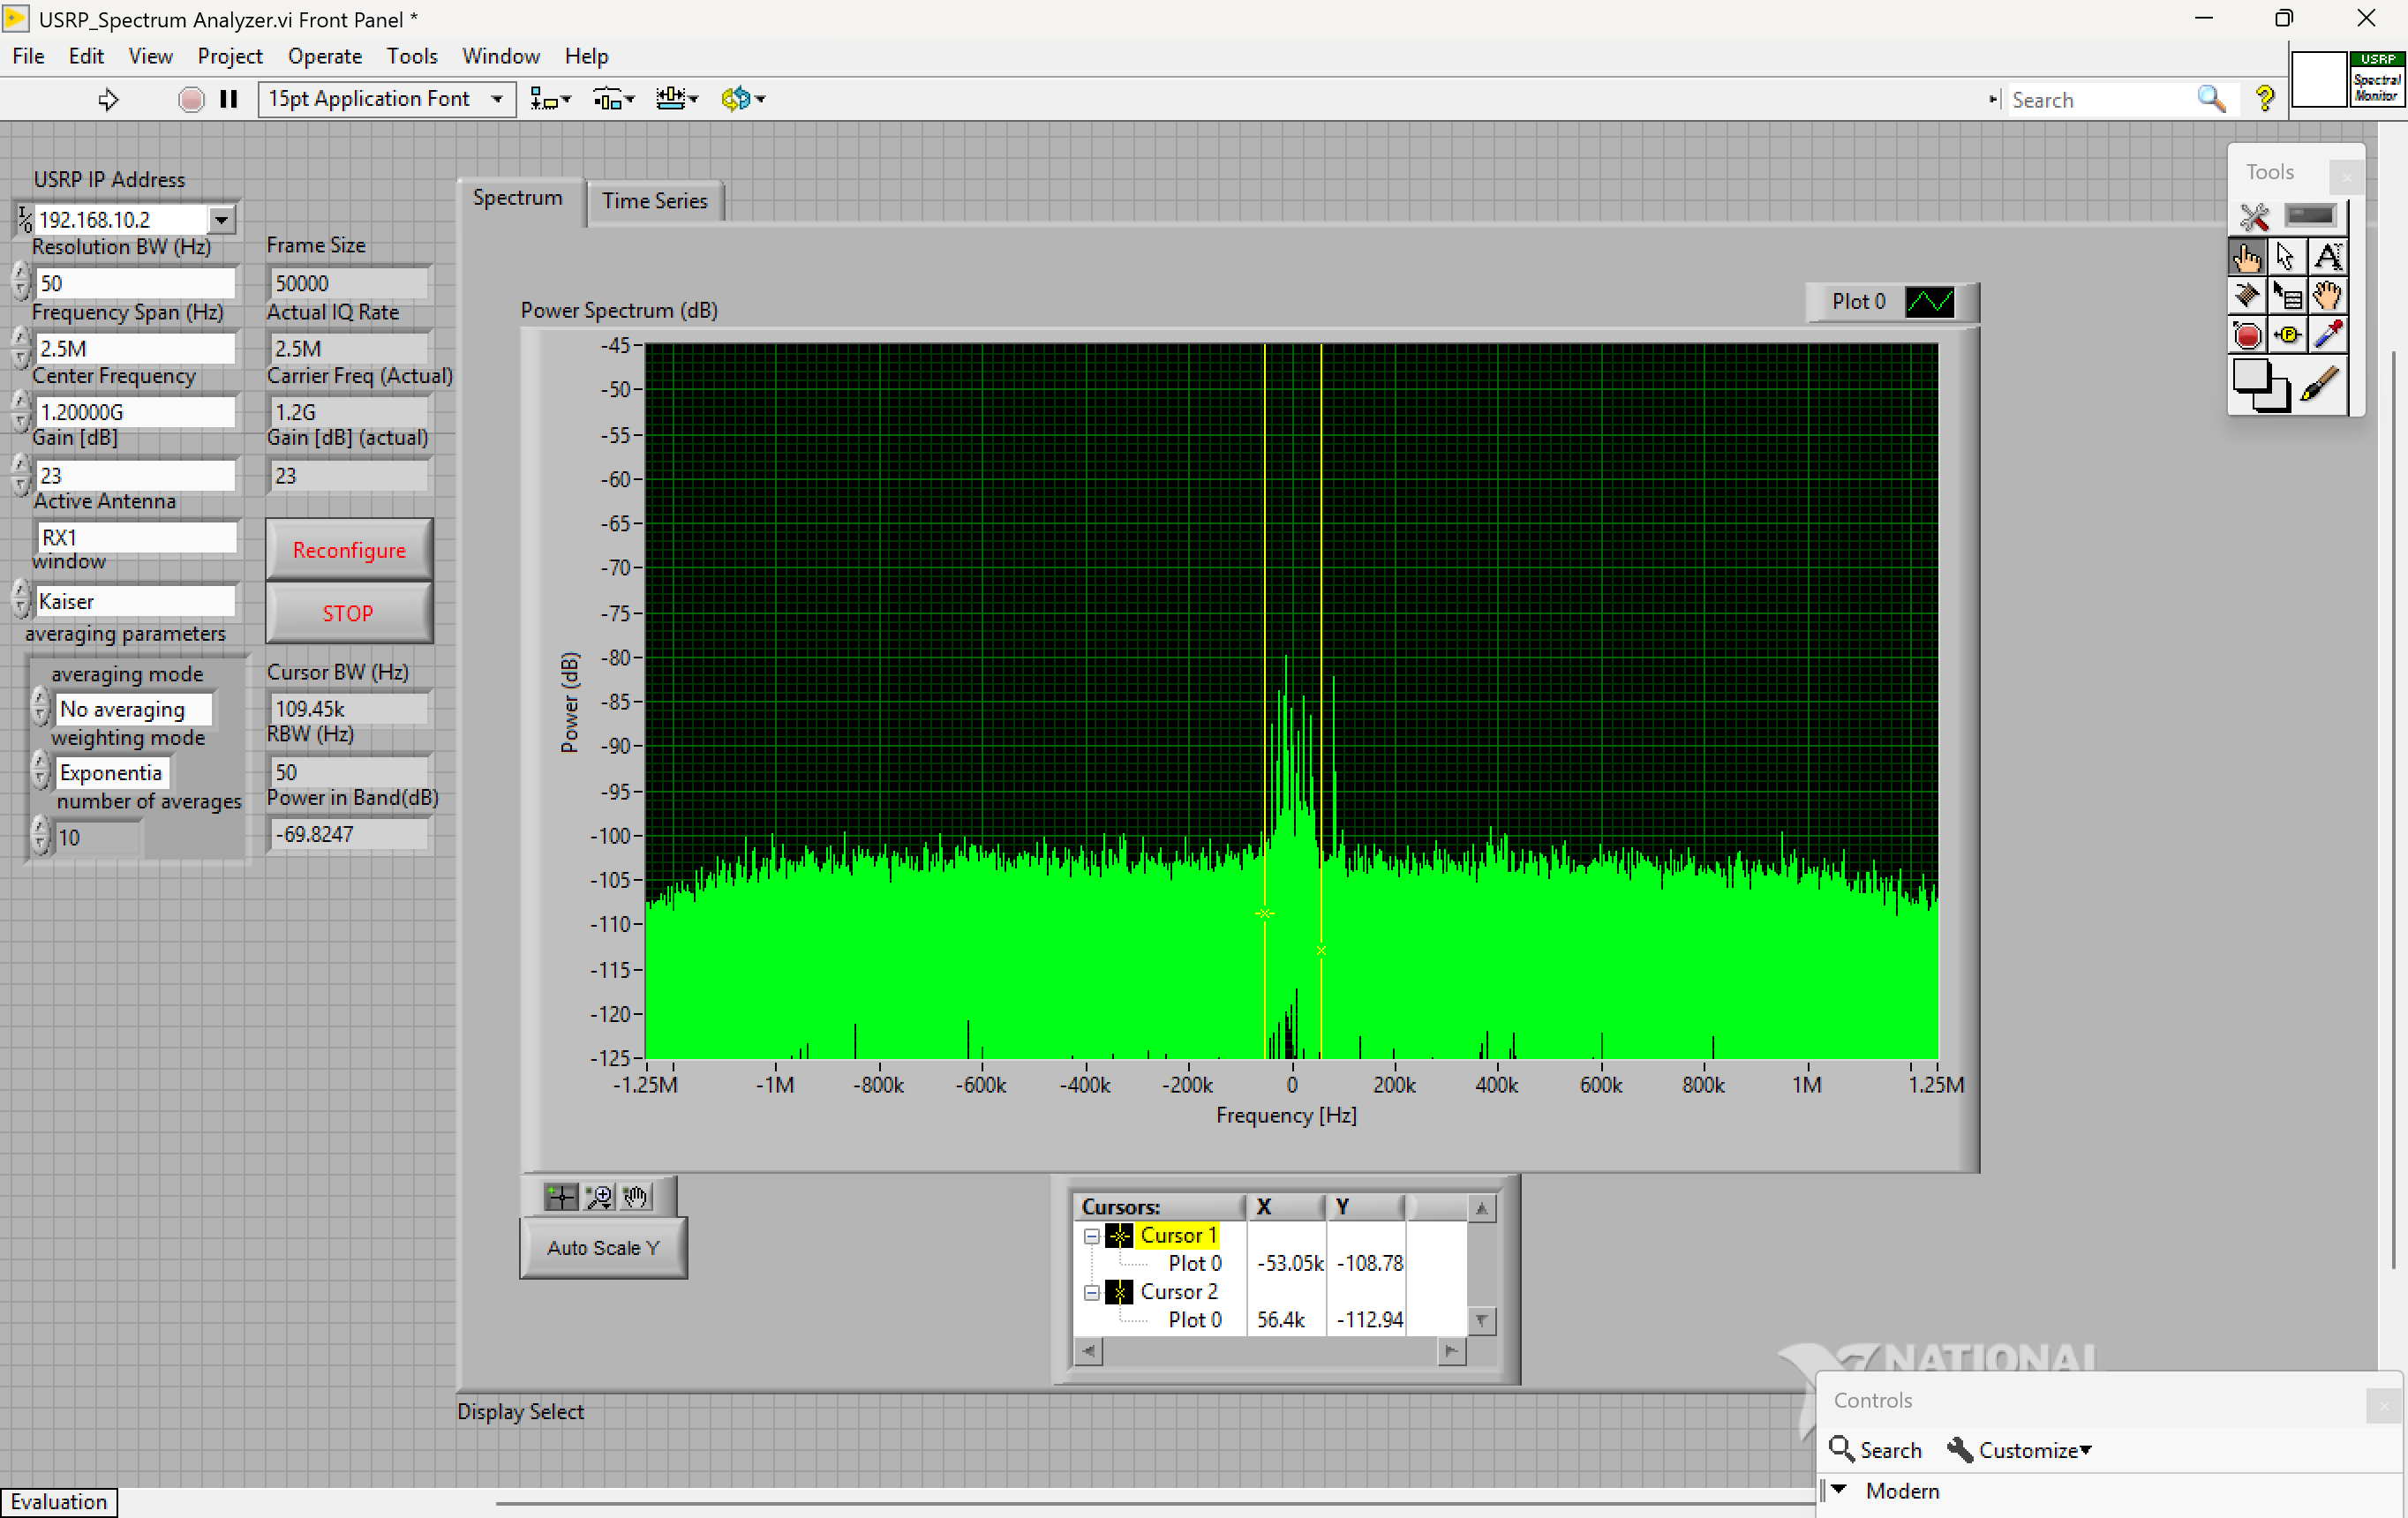
\includegraphics[width=0.7\textwidth]
   {../lab_ss/WES268B_Lab6_Part1-1-6_root-raised_measured-109khz_filter-parameter-0.png}
   \caption{1.1.6 - RX RRC, $\beta = 0$}
\end{figure}
\par
\begin{figure}[H]
   \centering
   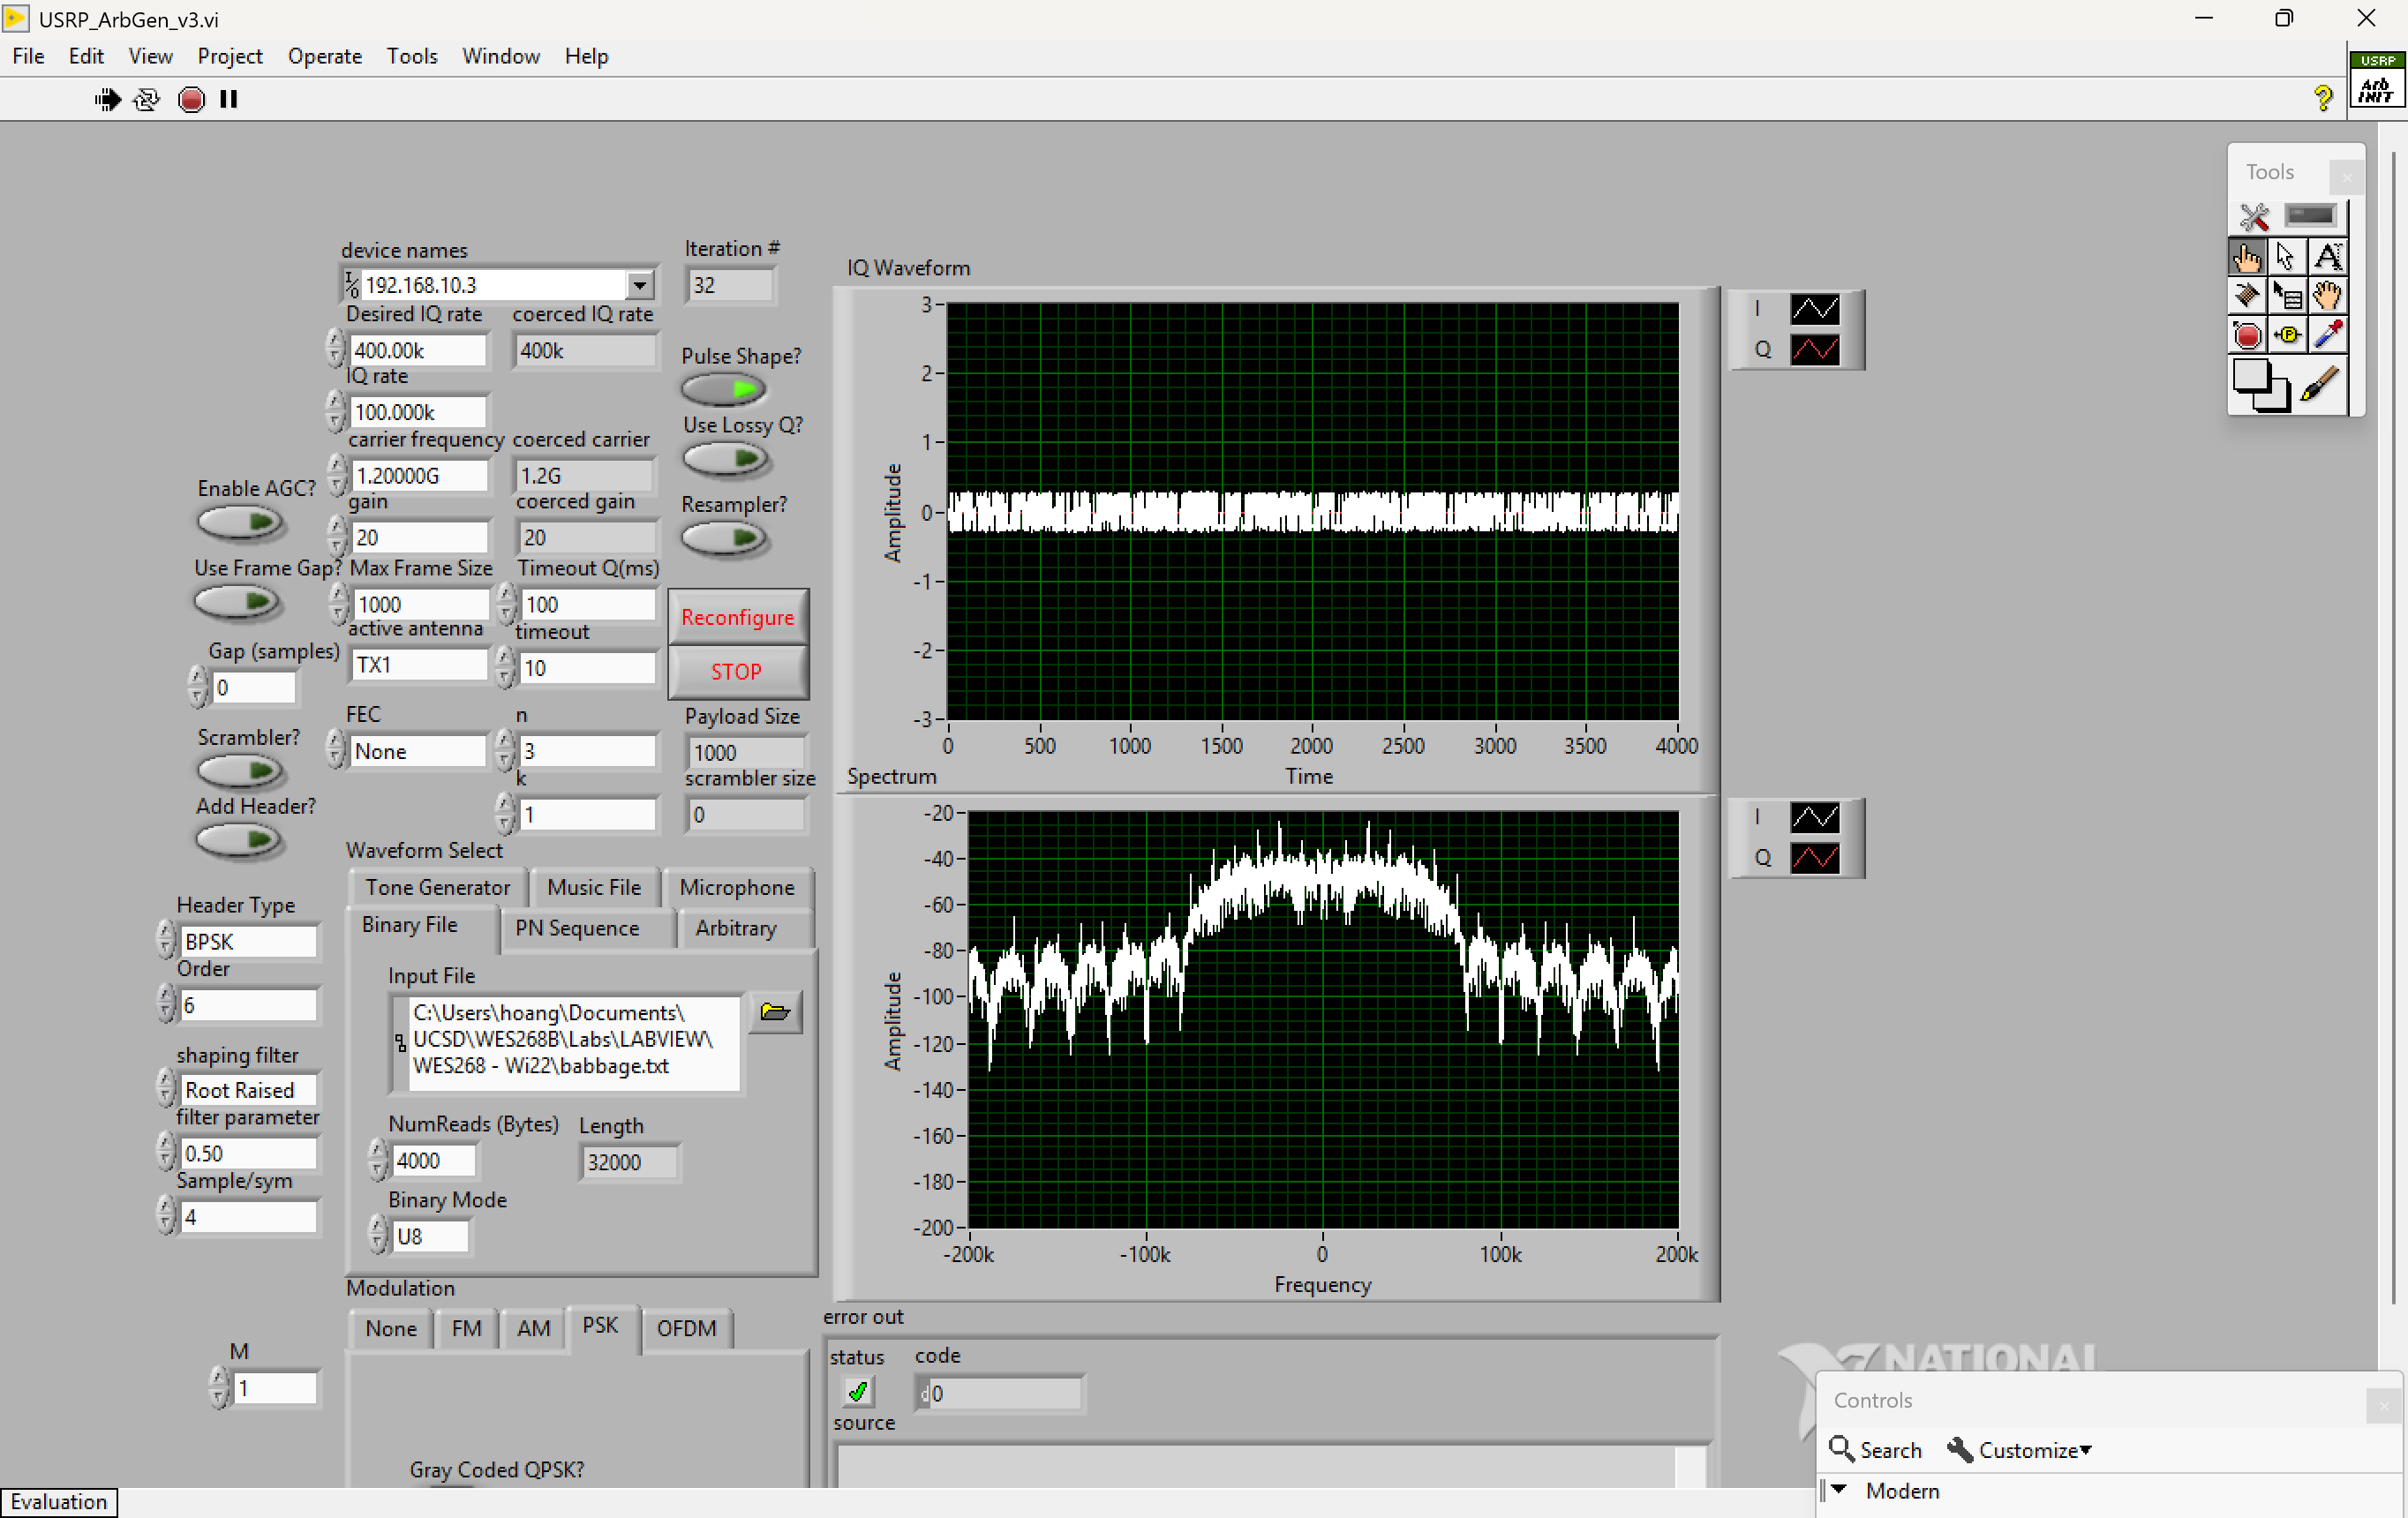
\includegraphics[width=0.7\textwidth]
   {../lab_ss/WES268B_Lab6_Part1-1-6_Tx_root-raised_filter-parameter-0p5.png}
   \caption{1.1.6 - TX RRC, $\beta = 0.5$}
\end{figure}
\par
\begin{figure}[H]
   \centering
   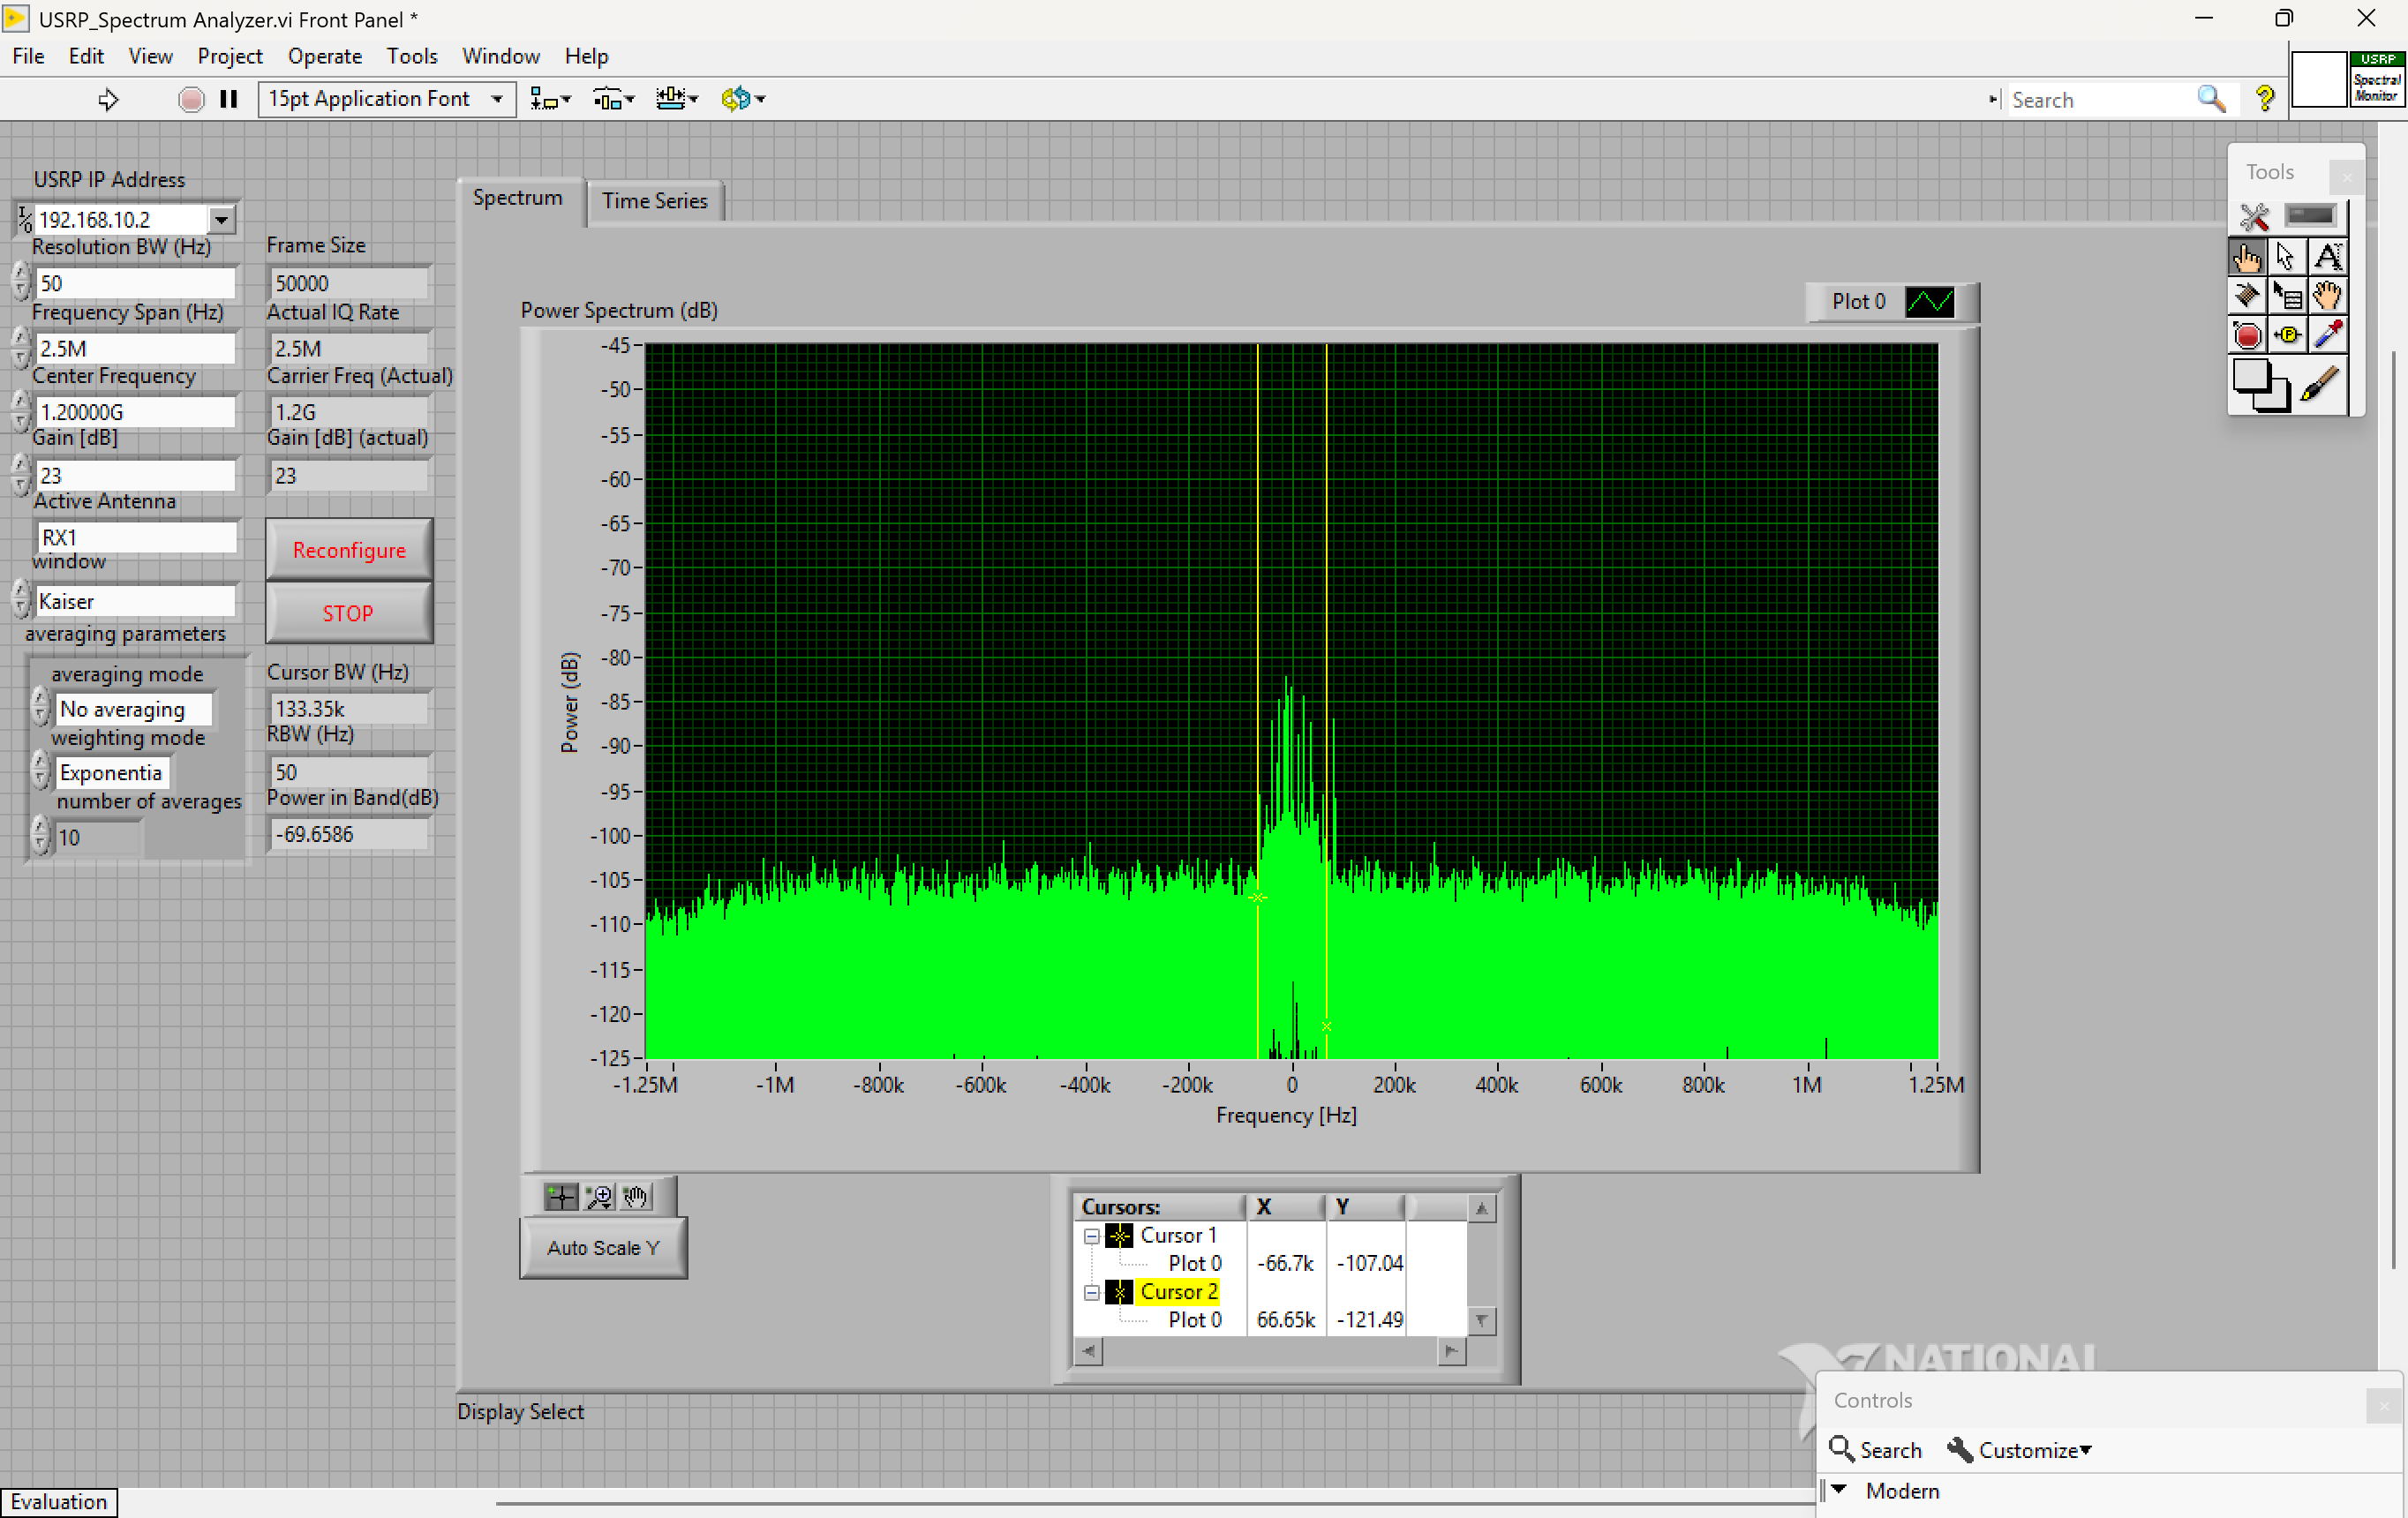
\includegraphics[width=0.7\textwidth]
   {../lab_ss/WES268B_Lab6_Part1-1-6_root-raised_measured-132khz_filter-parameter-0p5.png}
   \caption{1.1.6 - RX RRC, $\beta = 0.5$}
\end{figure}
\par
\begin{figure}[H]
   \centering
   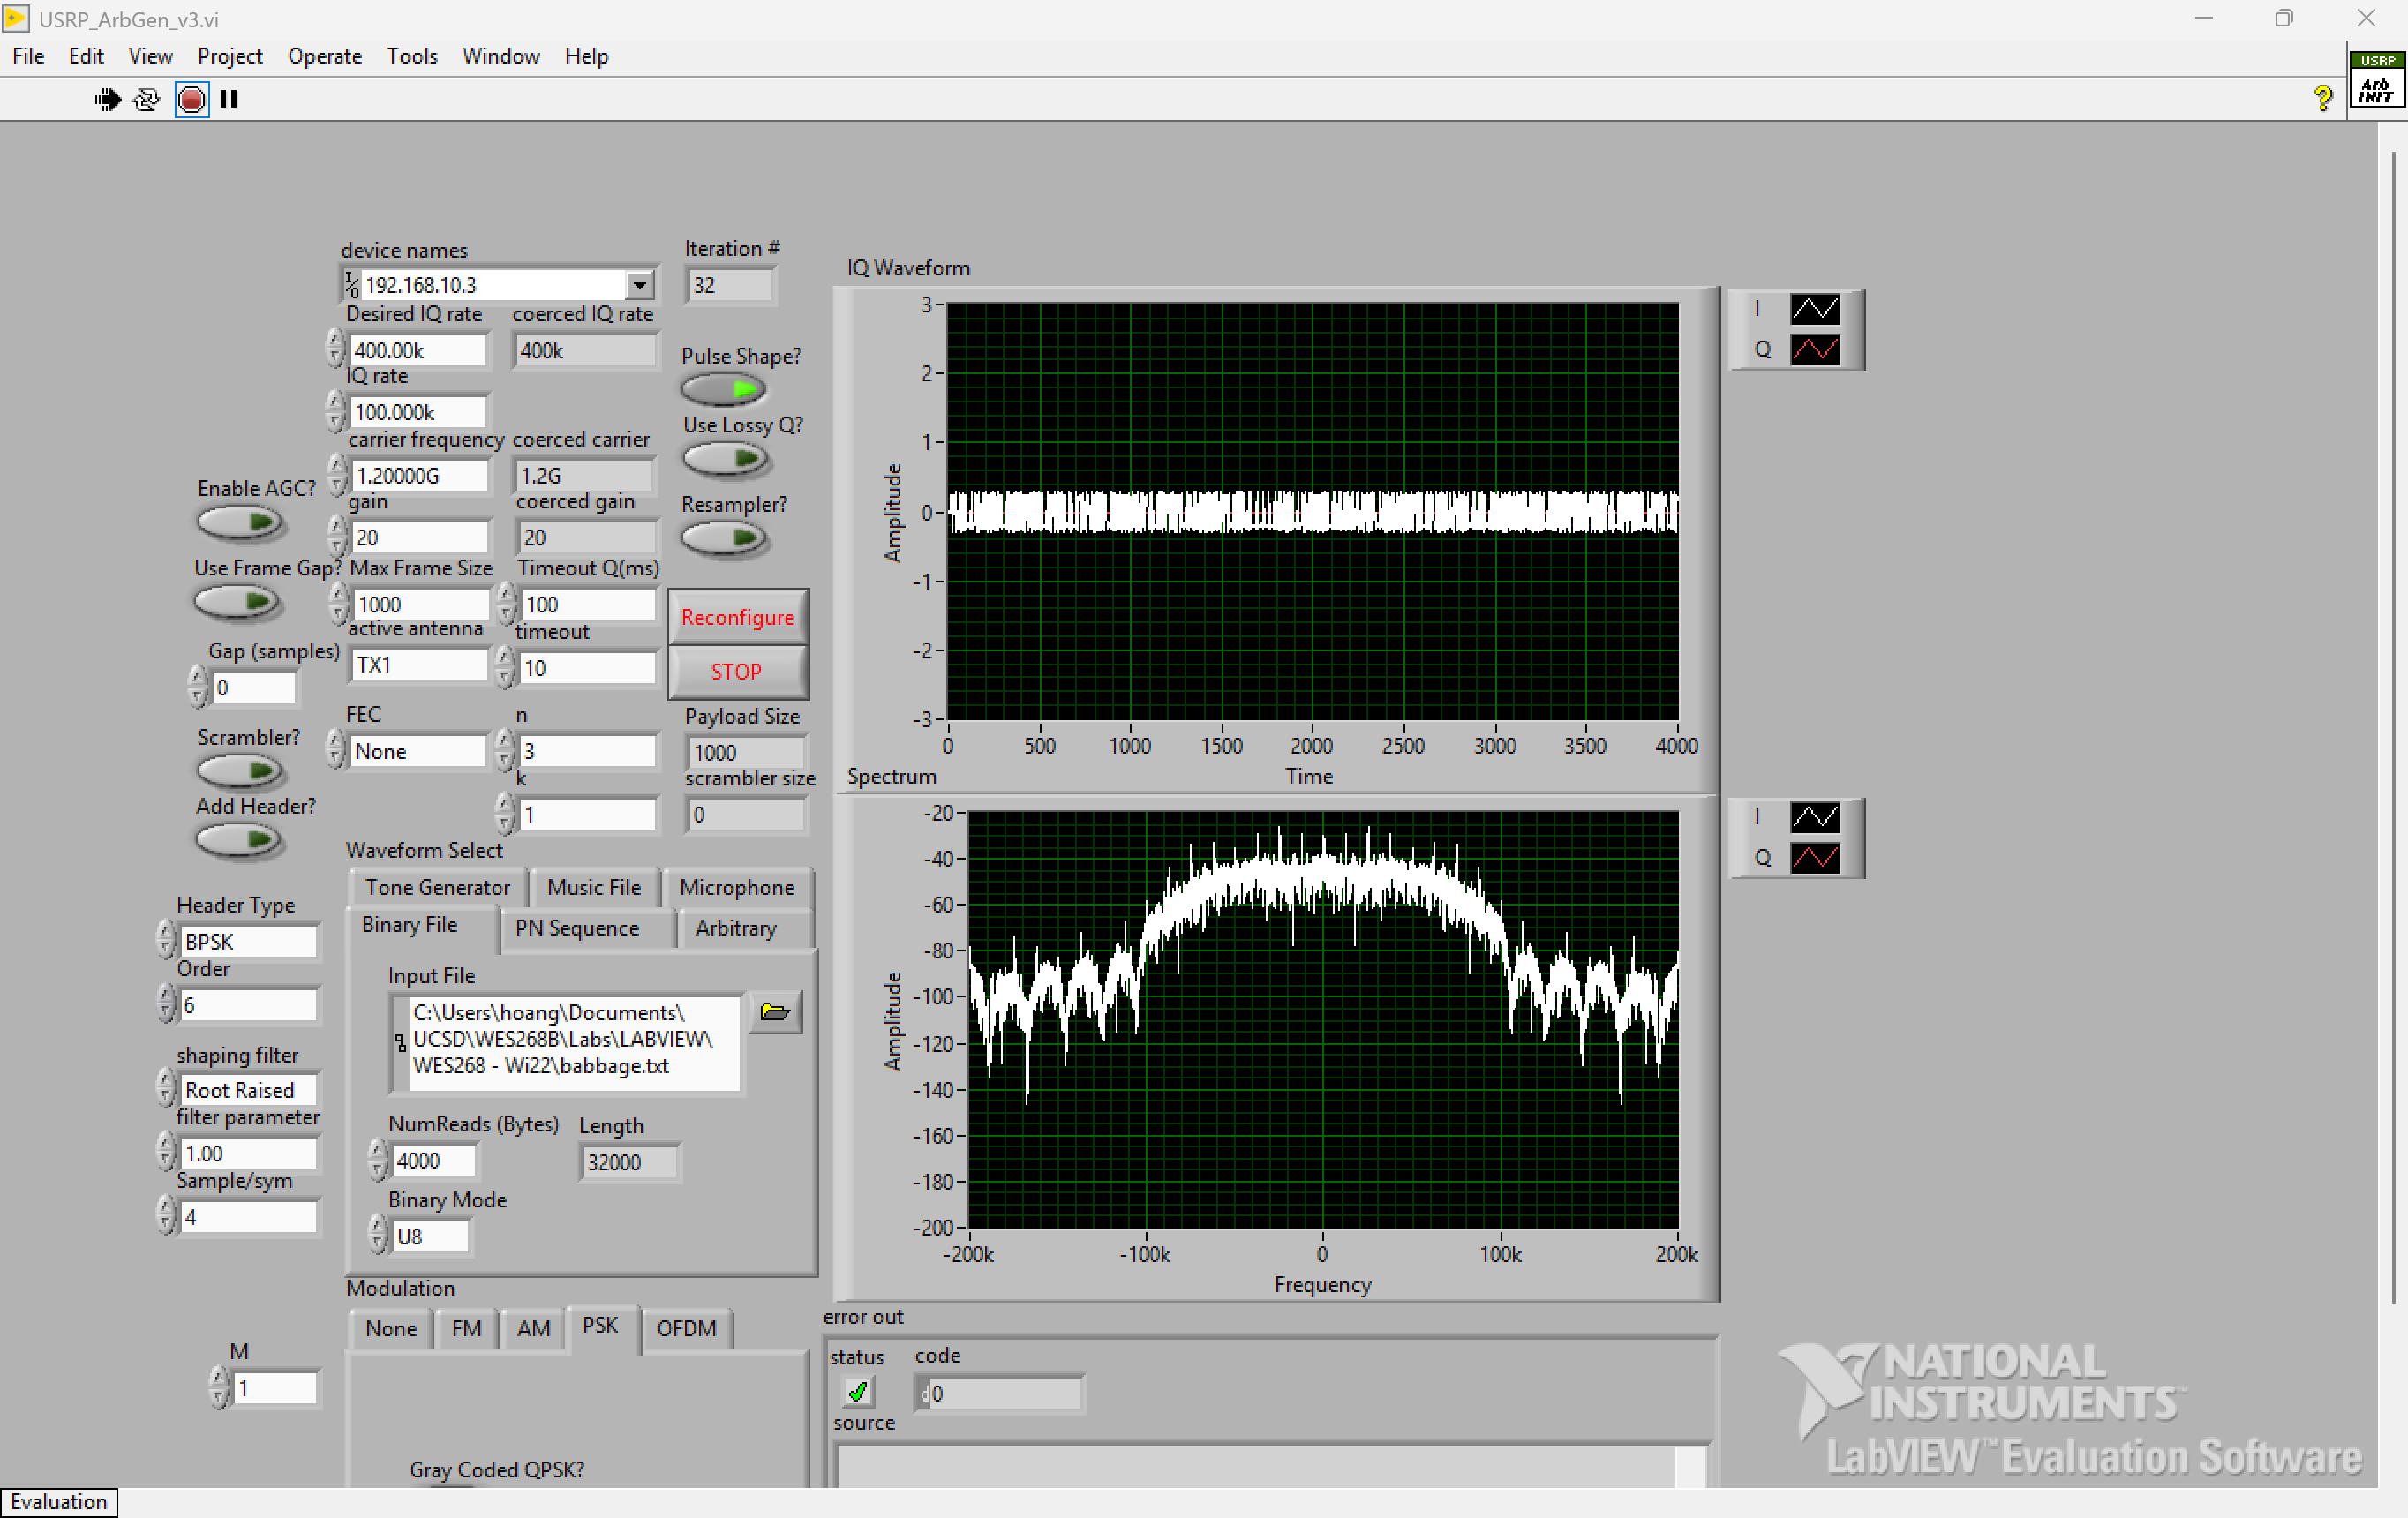
\includegraphics[width=0.7\textwidth]
   {../lab_ss/WES268B_Lab6_Part1-1-6_Tx_root-raised_filter-parameter-1.png}
   \caption{1.1.6 - TX RRC, $\beta = 1$}
\end{figure}
\par
\begin{figure}[H]
   \centering
   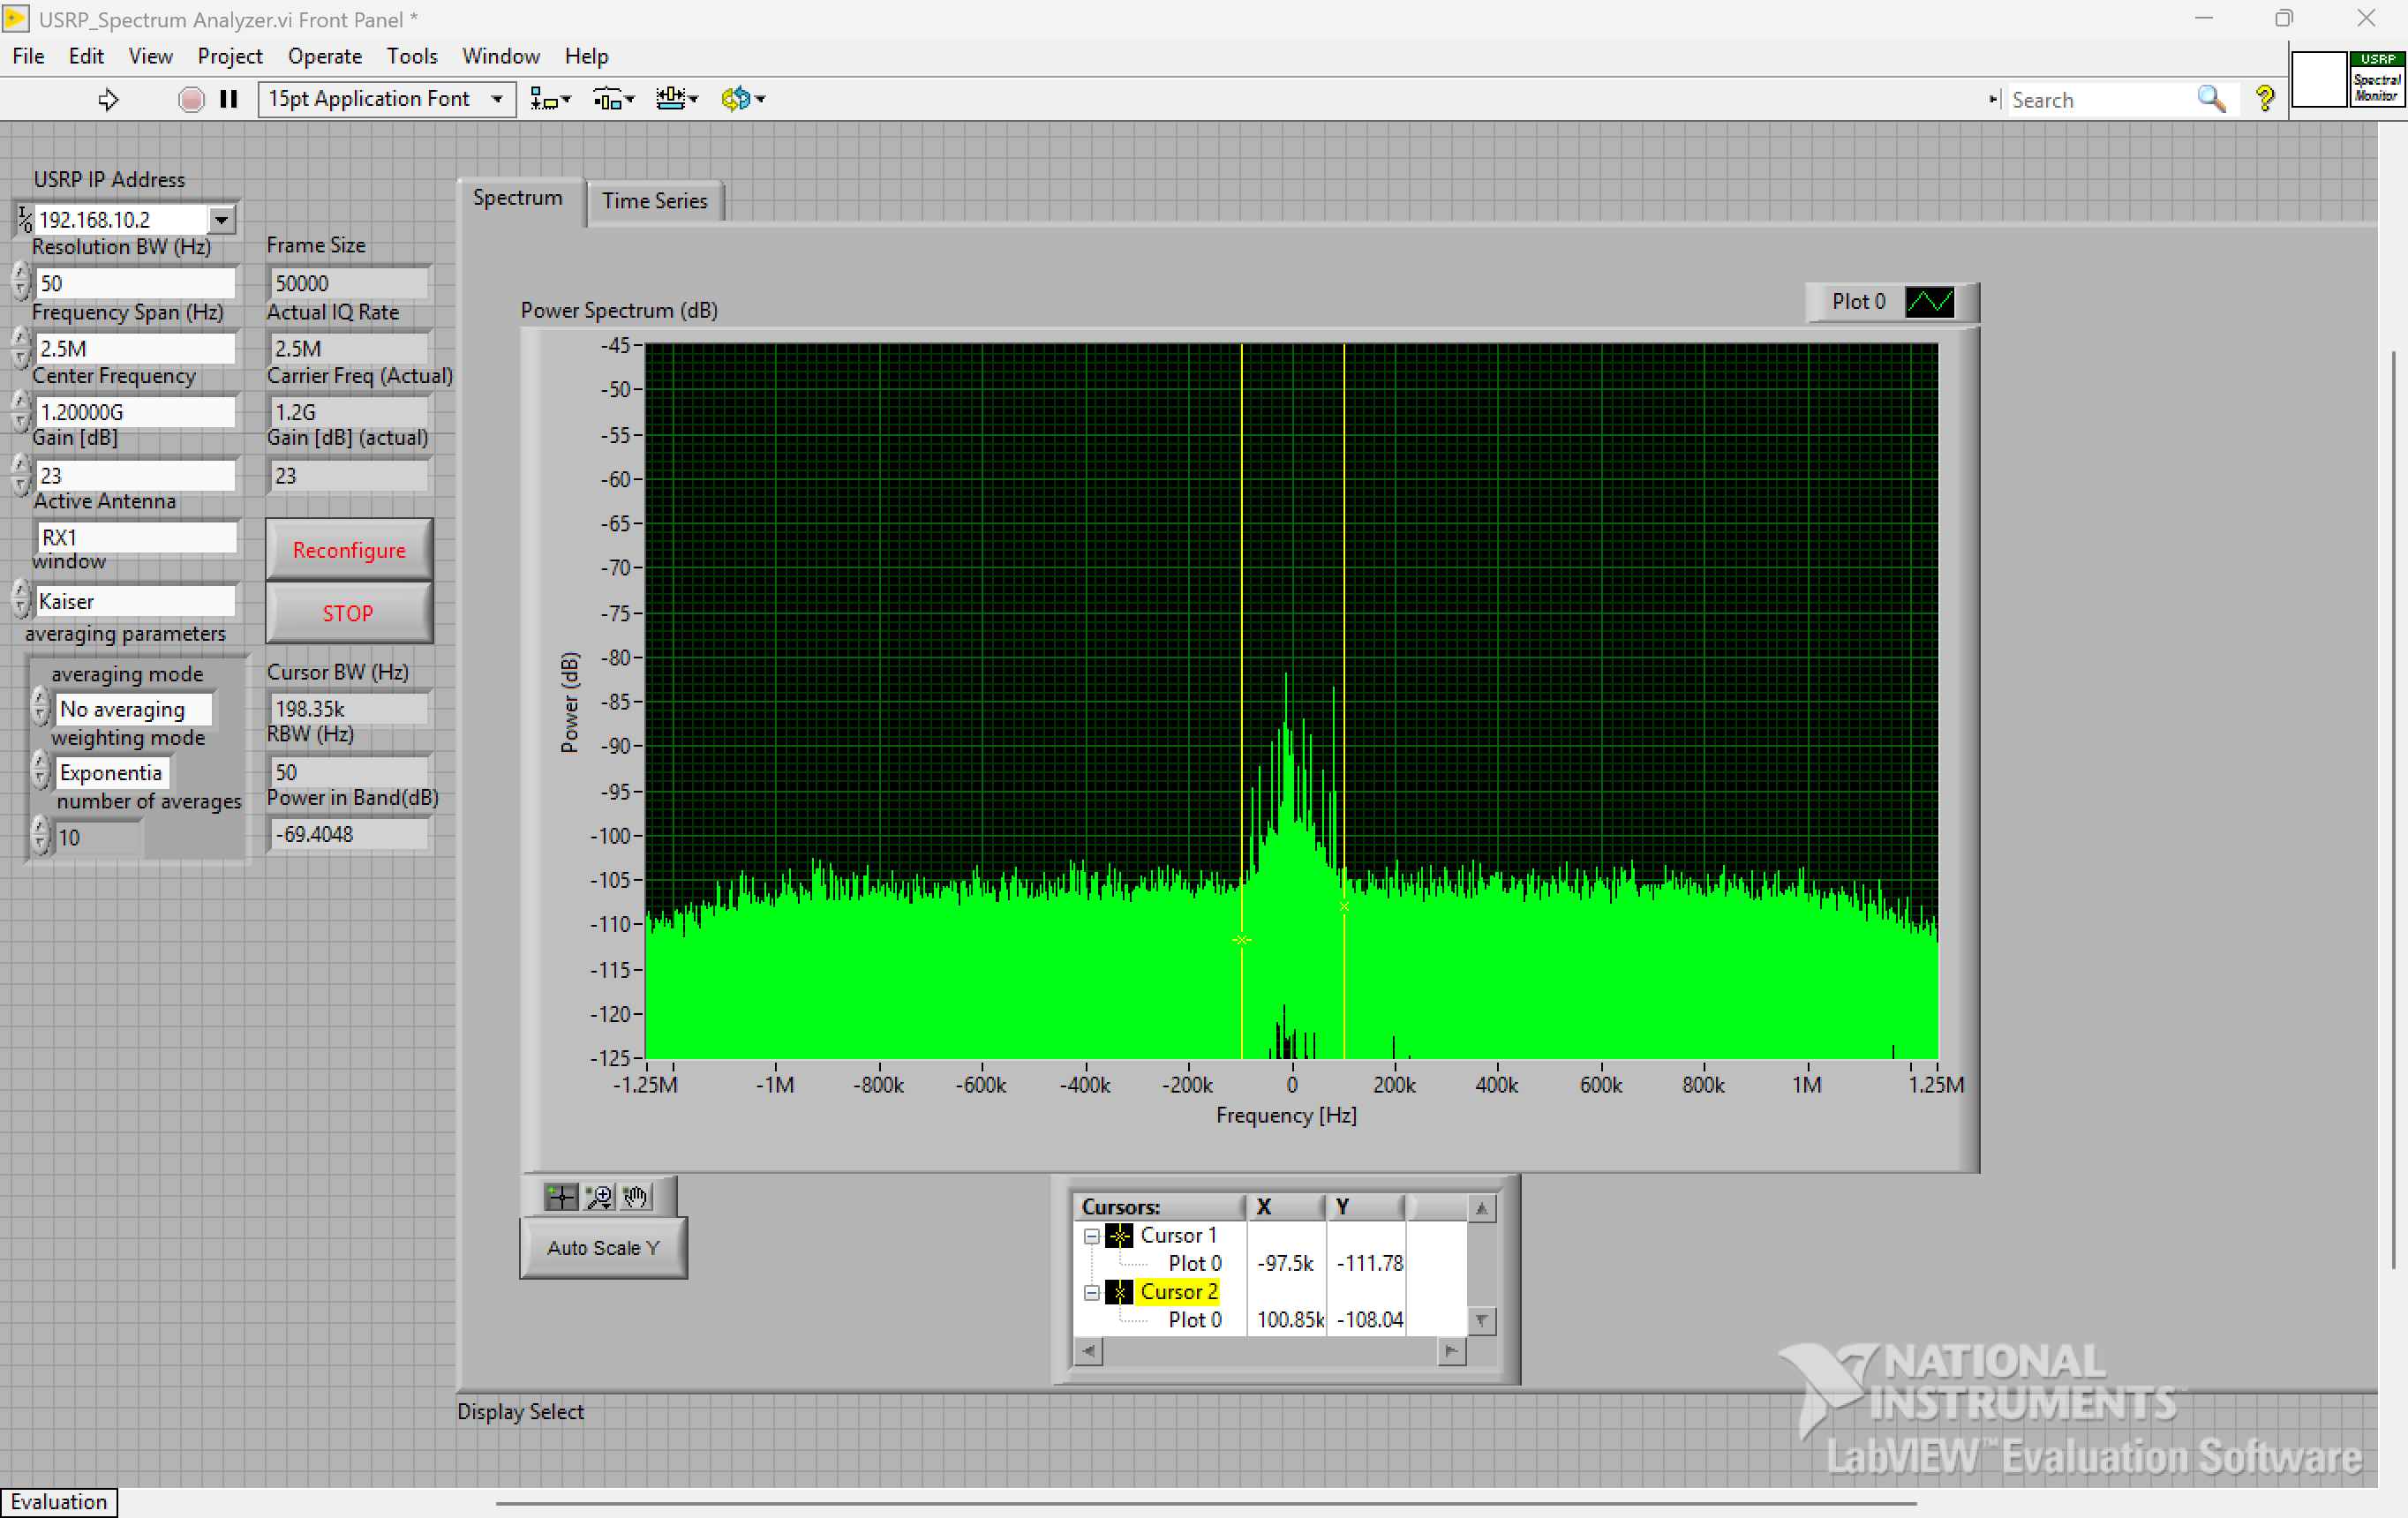
\includegraphics[width=0.7\textwidth]
   {../lab_ss/WES268B_Lab6_Part1-1-6_root-raised_measured-197khz_filter-parameter-1.png}
   \caption{1.1.6 - RX RRC, $\beta = 1$}
\end{figure}
\par

% 1.1.7
\subsubsection{}
\begin{figure}[H]
   \centering
   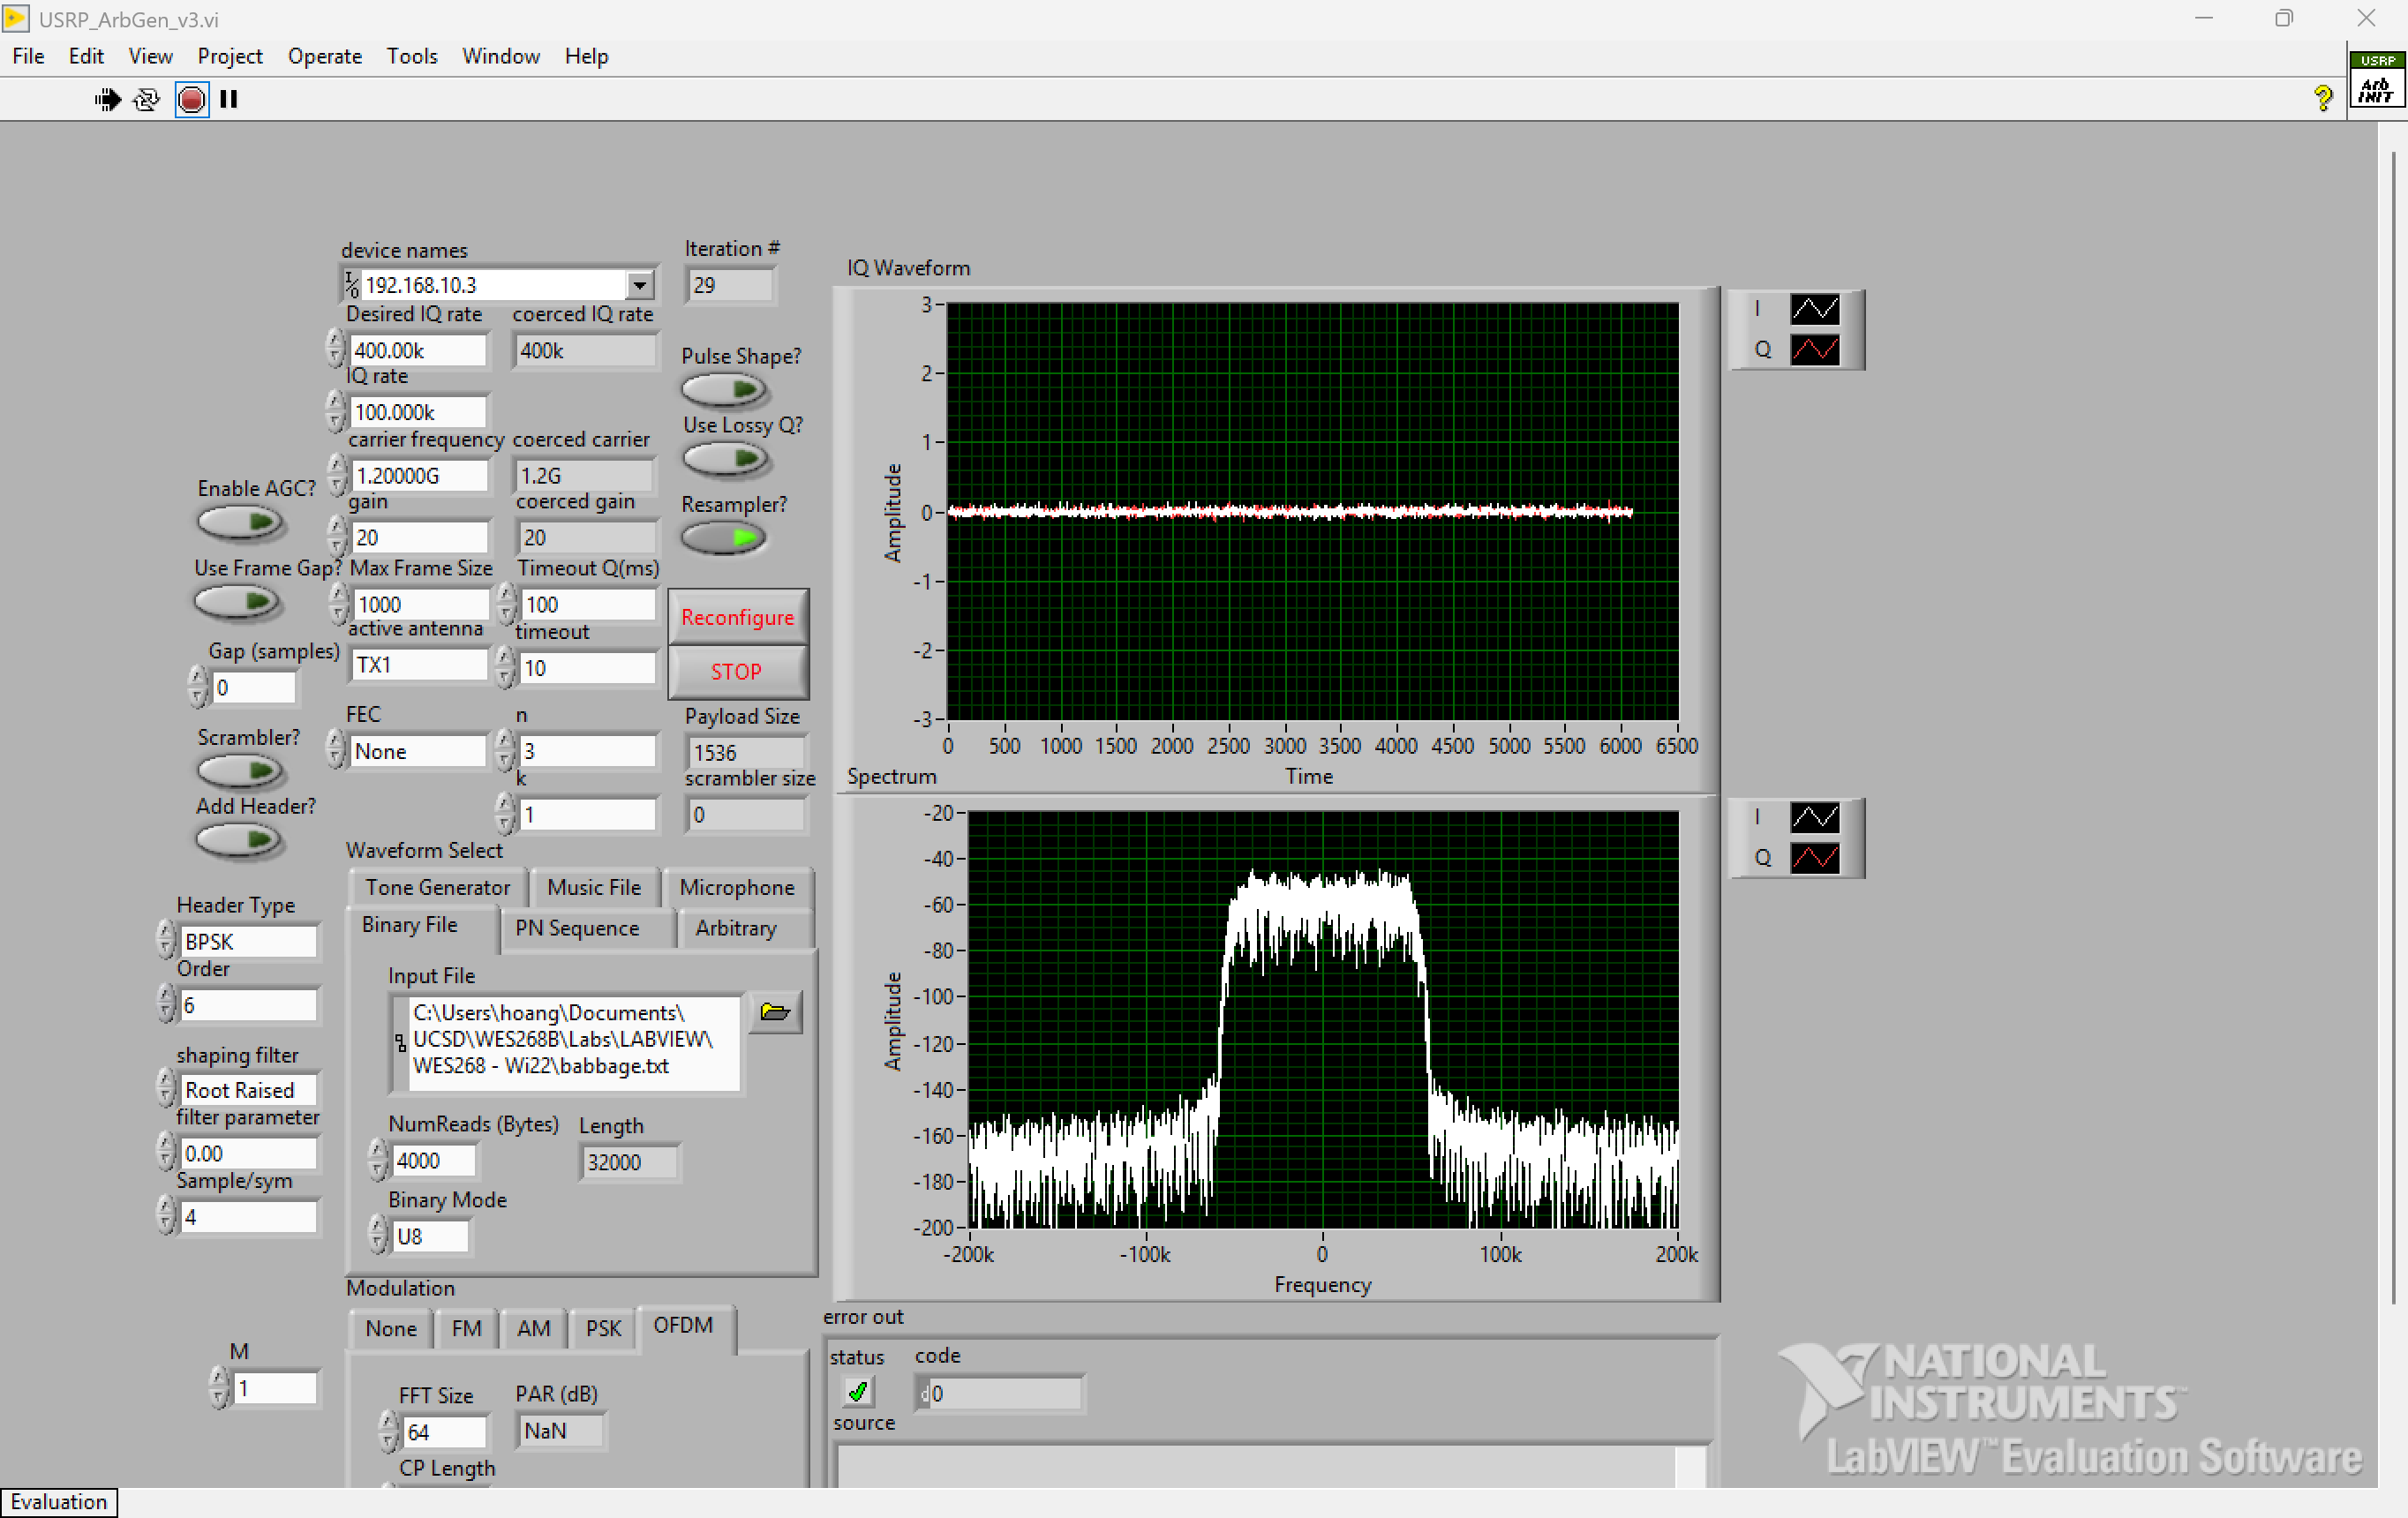
\includegraphics[width=0.7\textwidth]
   {../lab_ss/WES268B_Lab6_Part1-1-7_Tx_OFDM_filter-parameter-0.png}
   \caption{1.1.7 - TX OFDM, $\beta = 0$}
\end{figure}
\par
\begin{figure}[H]
   \centering
   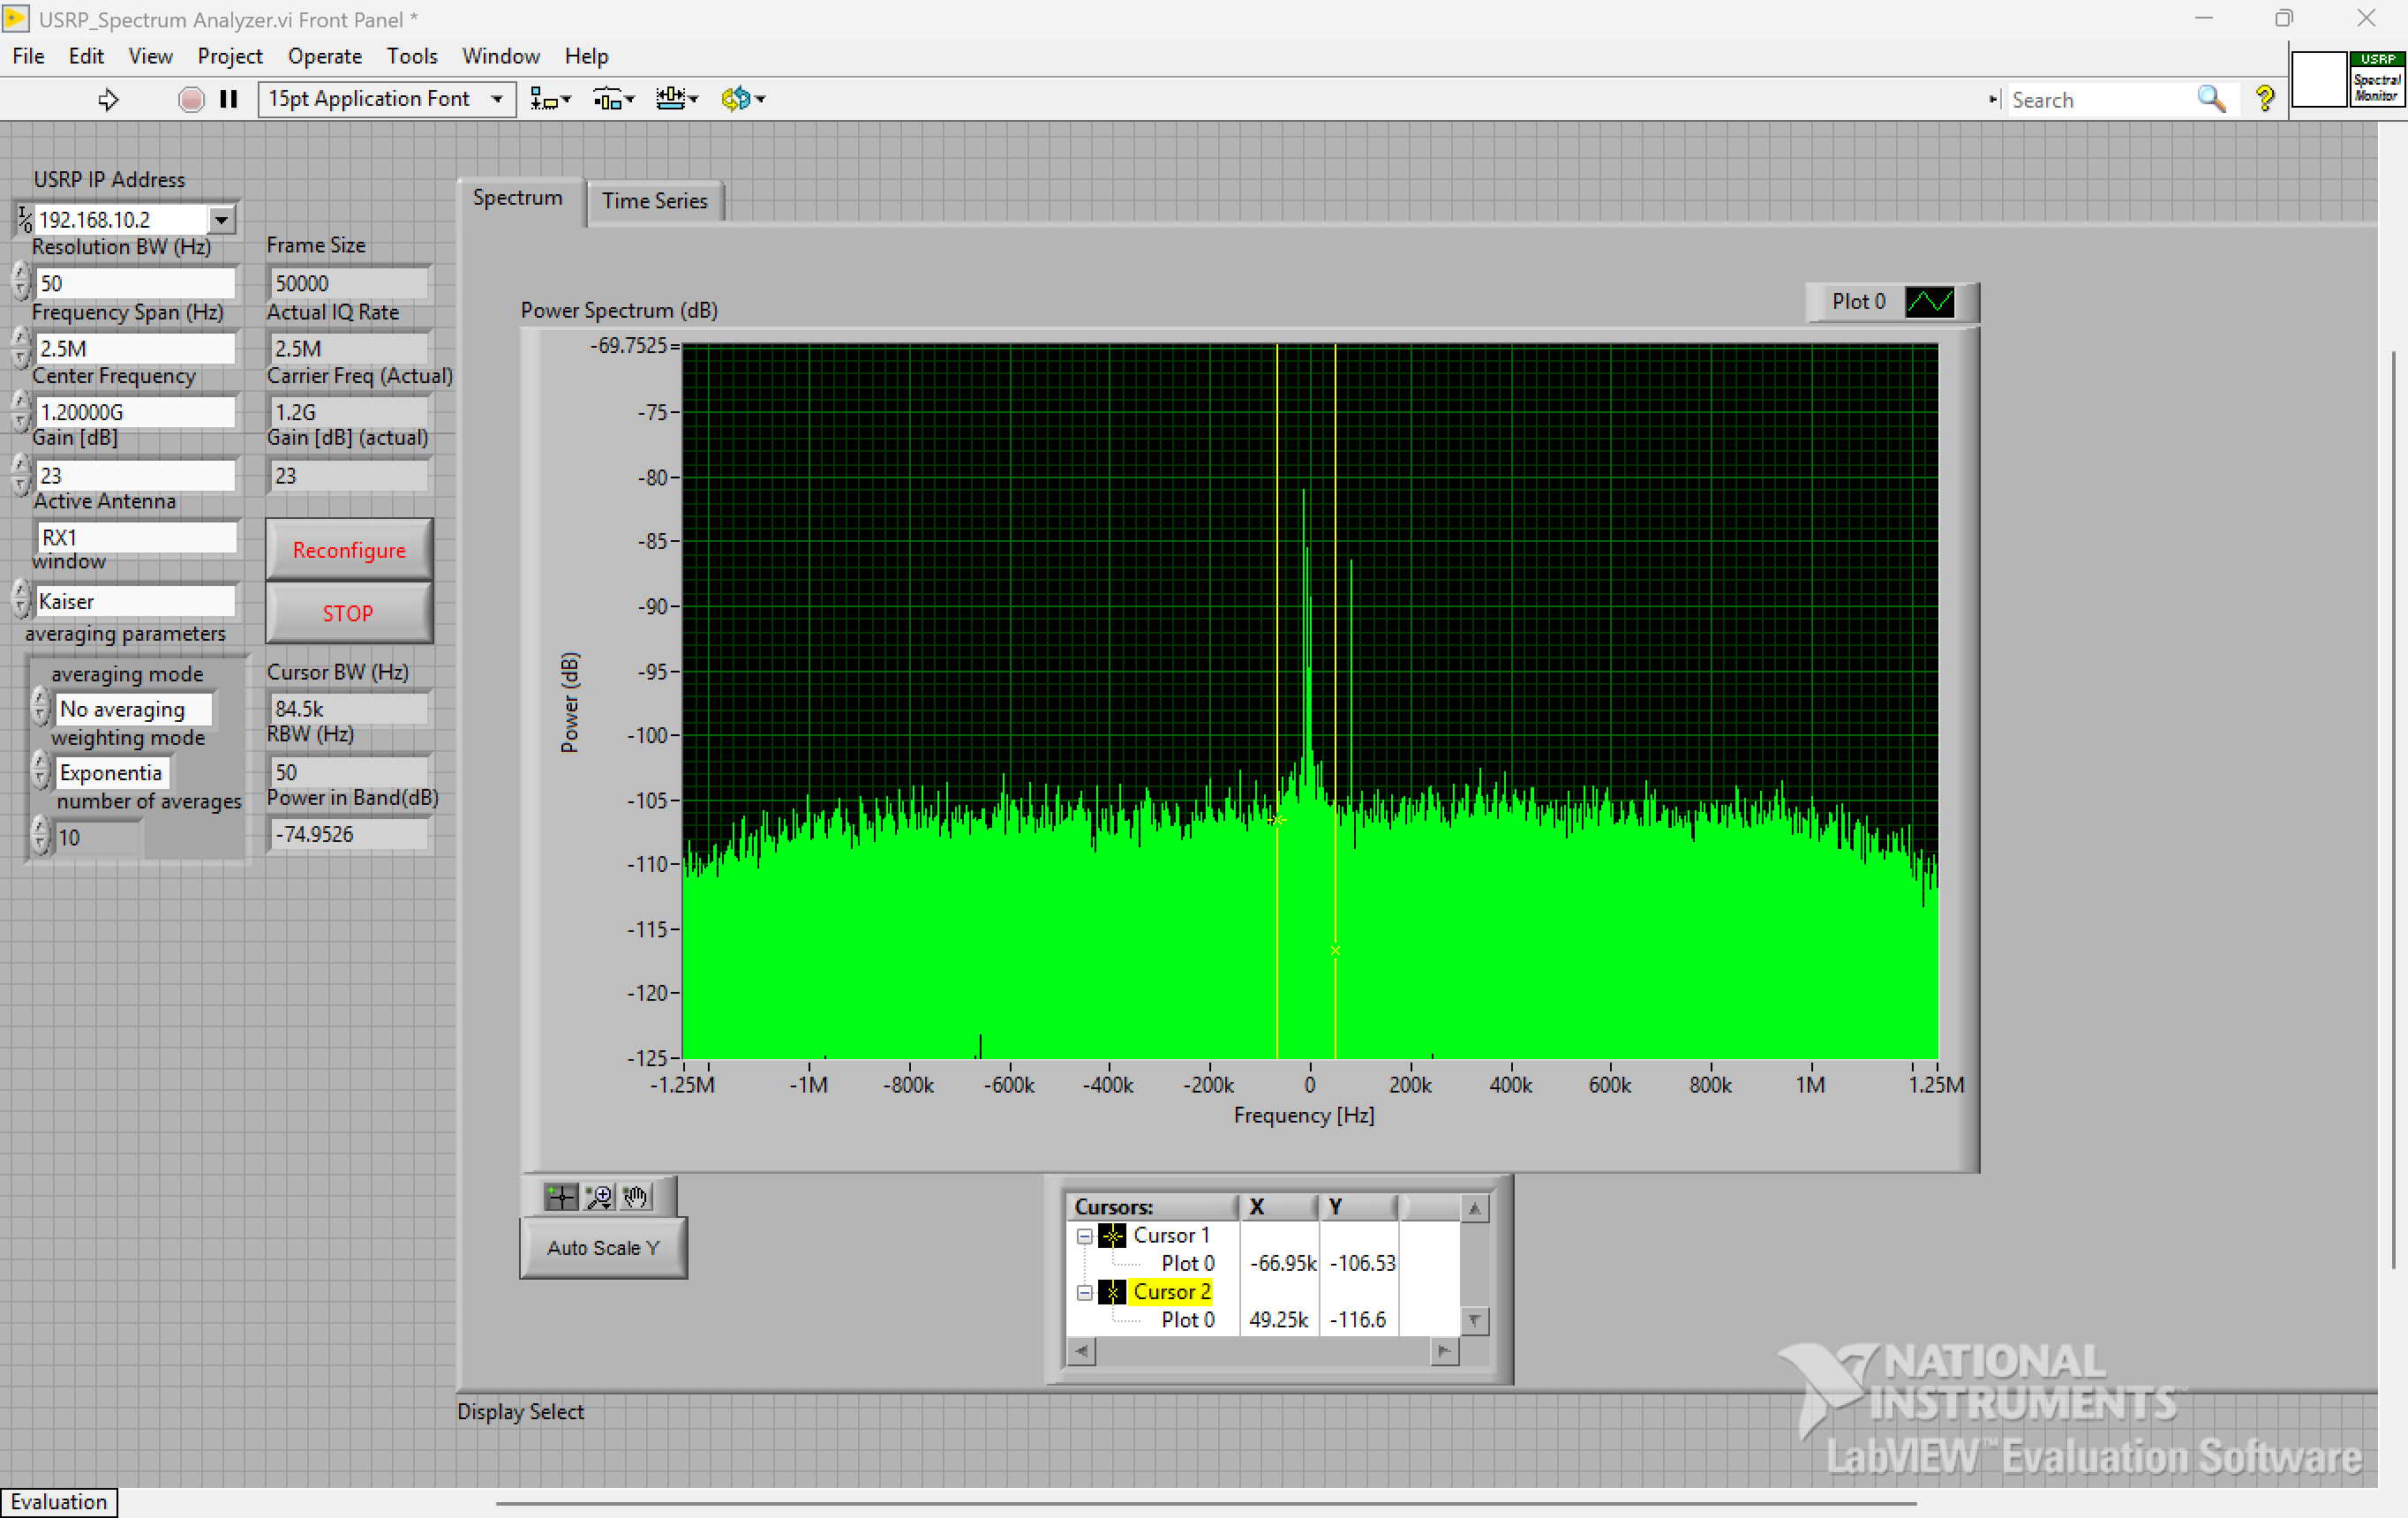
\includegraphics[width=0.7\textwidth]
   {../lab_ss/WES268B_Lab6_Part1-1-7_OFDM_measured-115khz_filter-parameter-0.png}
   \caption{1.1.7 - RX OFDM, $\beta = 0$}
\end{figure}
\par
\begin{figure}[H]
   \centering
   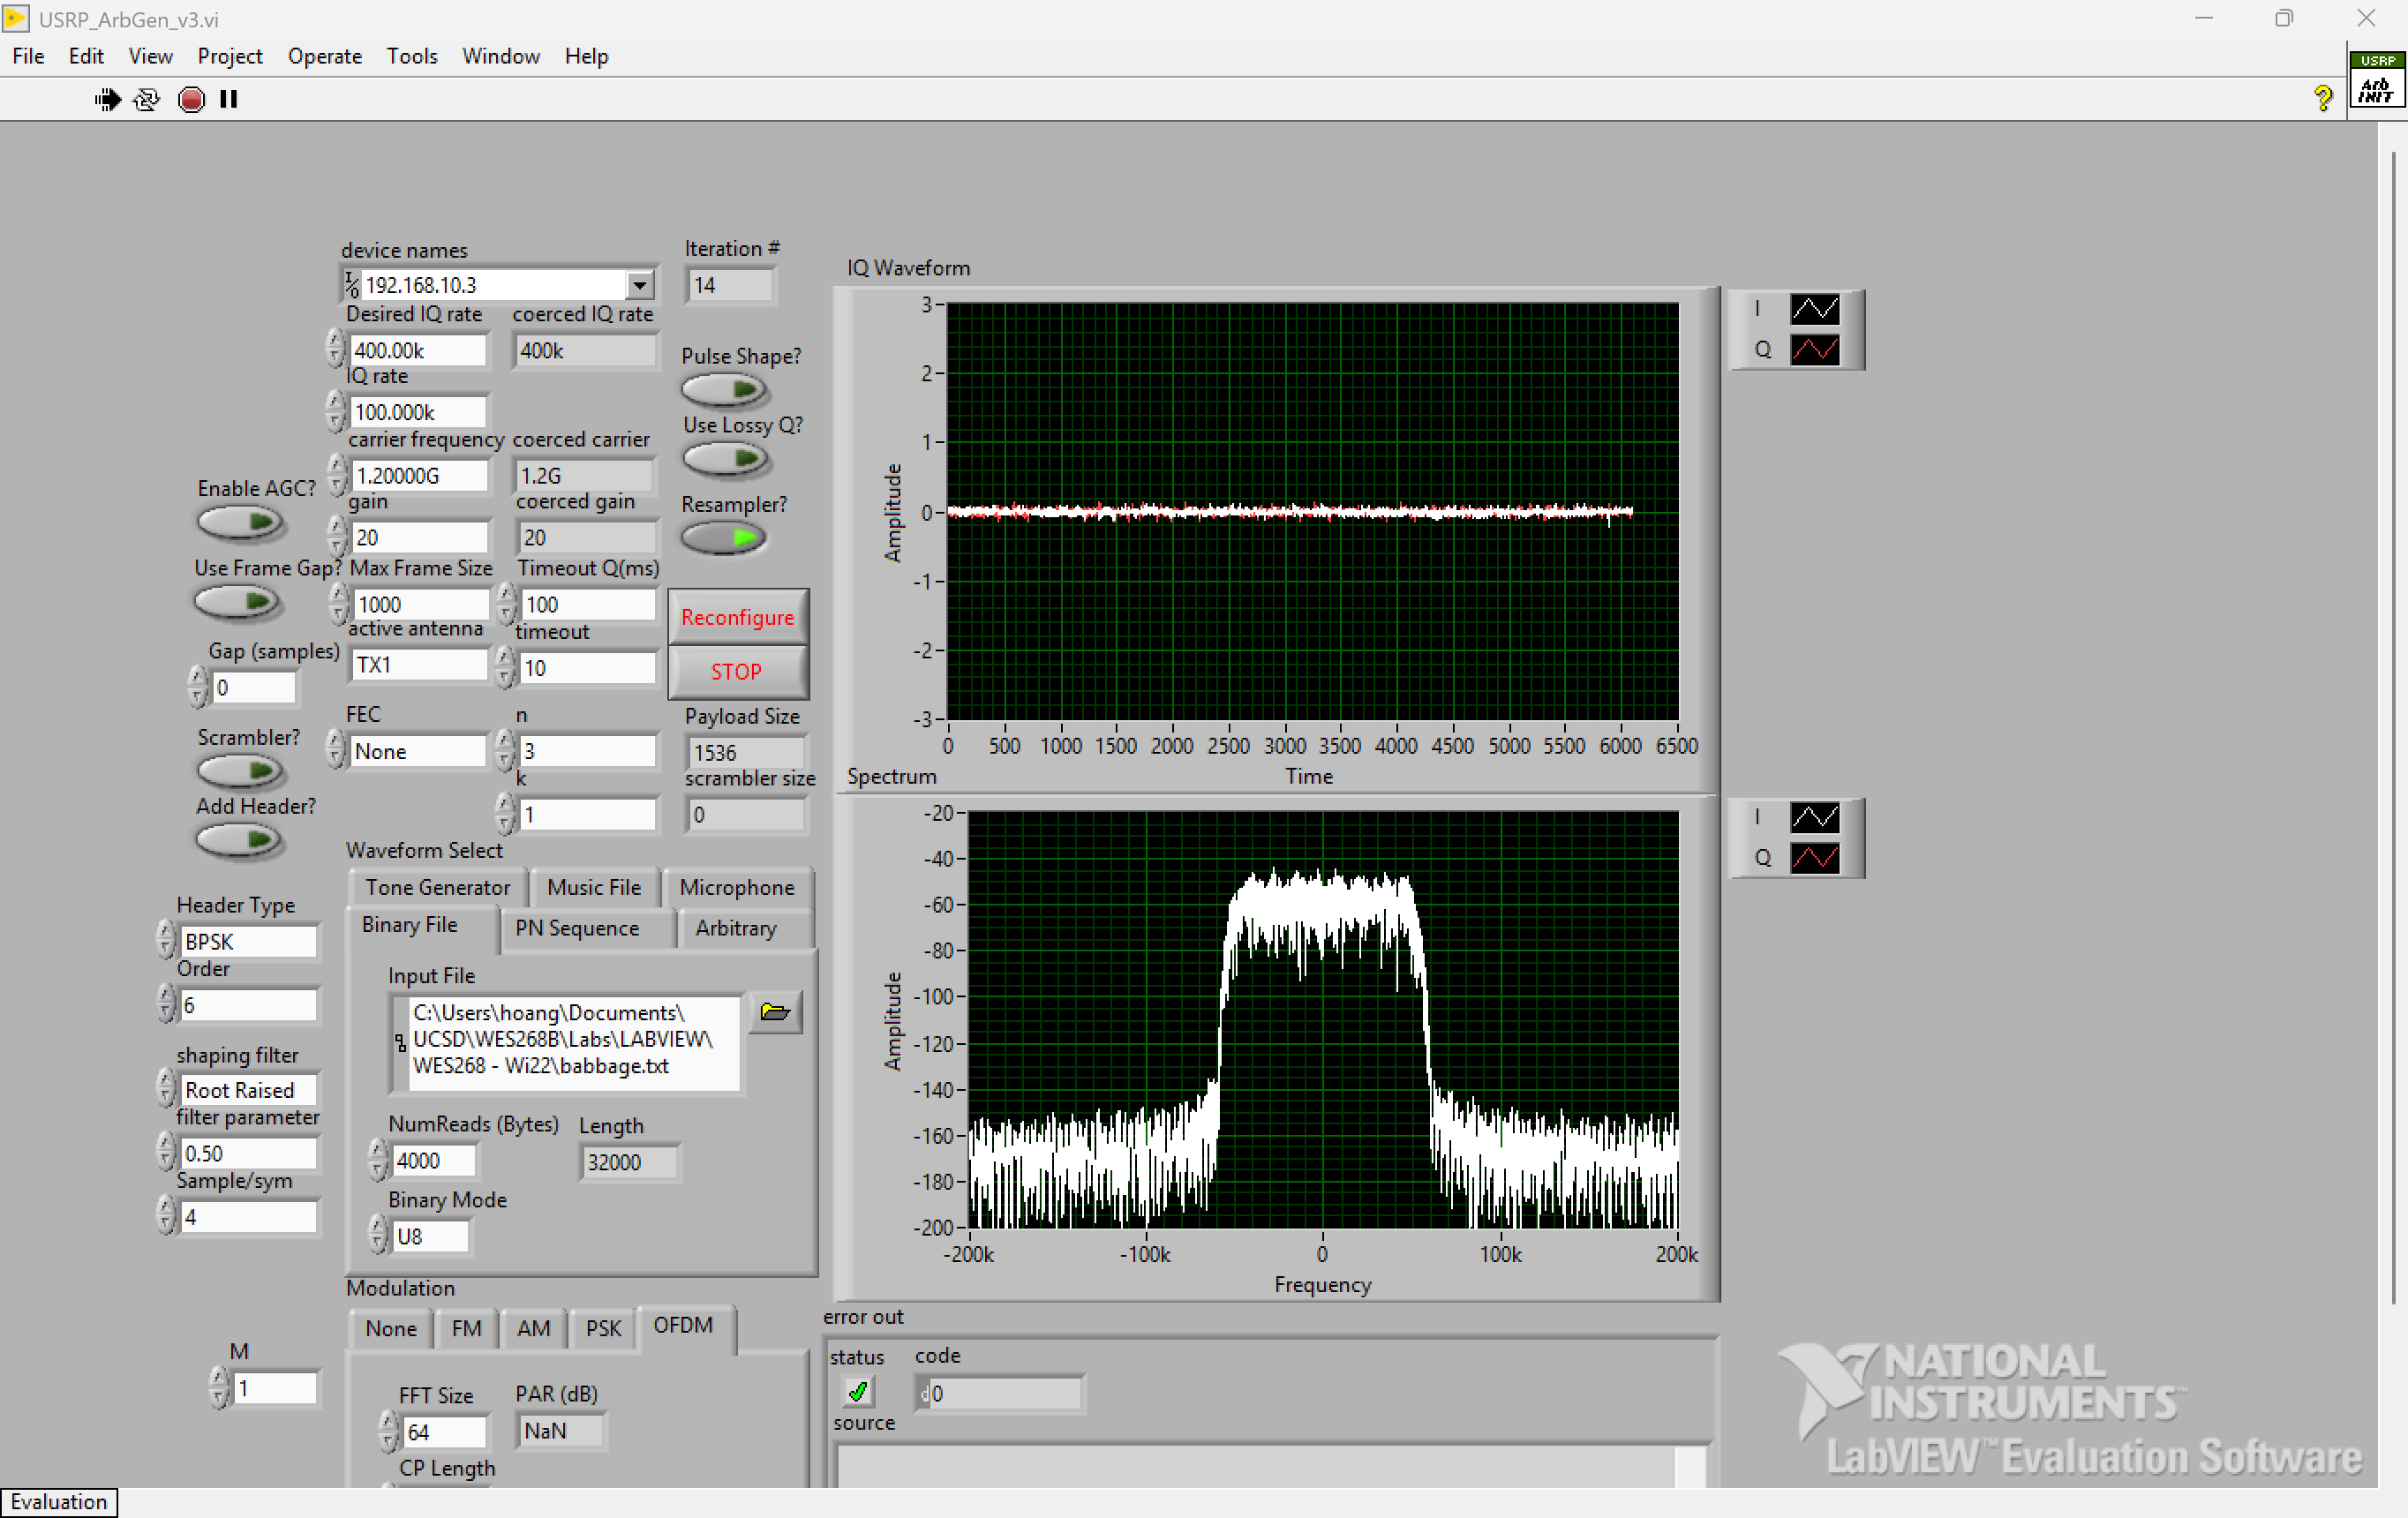
\includegraphics[width=0.7\textwidth]
   {../lab_ss/WES268B_Lab6_Part1-1-7_Tx_OFDM_filter-parameter-0p5.png}
   \caption{1.1.7 - TX OFDM, $\beta = 0.5$}
\end{figure}
\par
\begin{figure}[H]
   \centering
   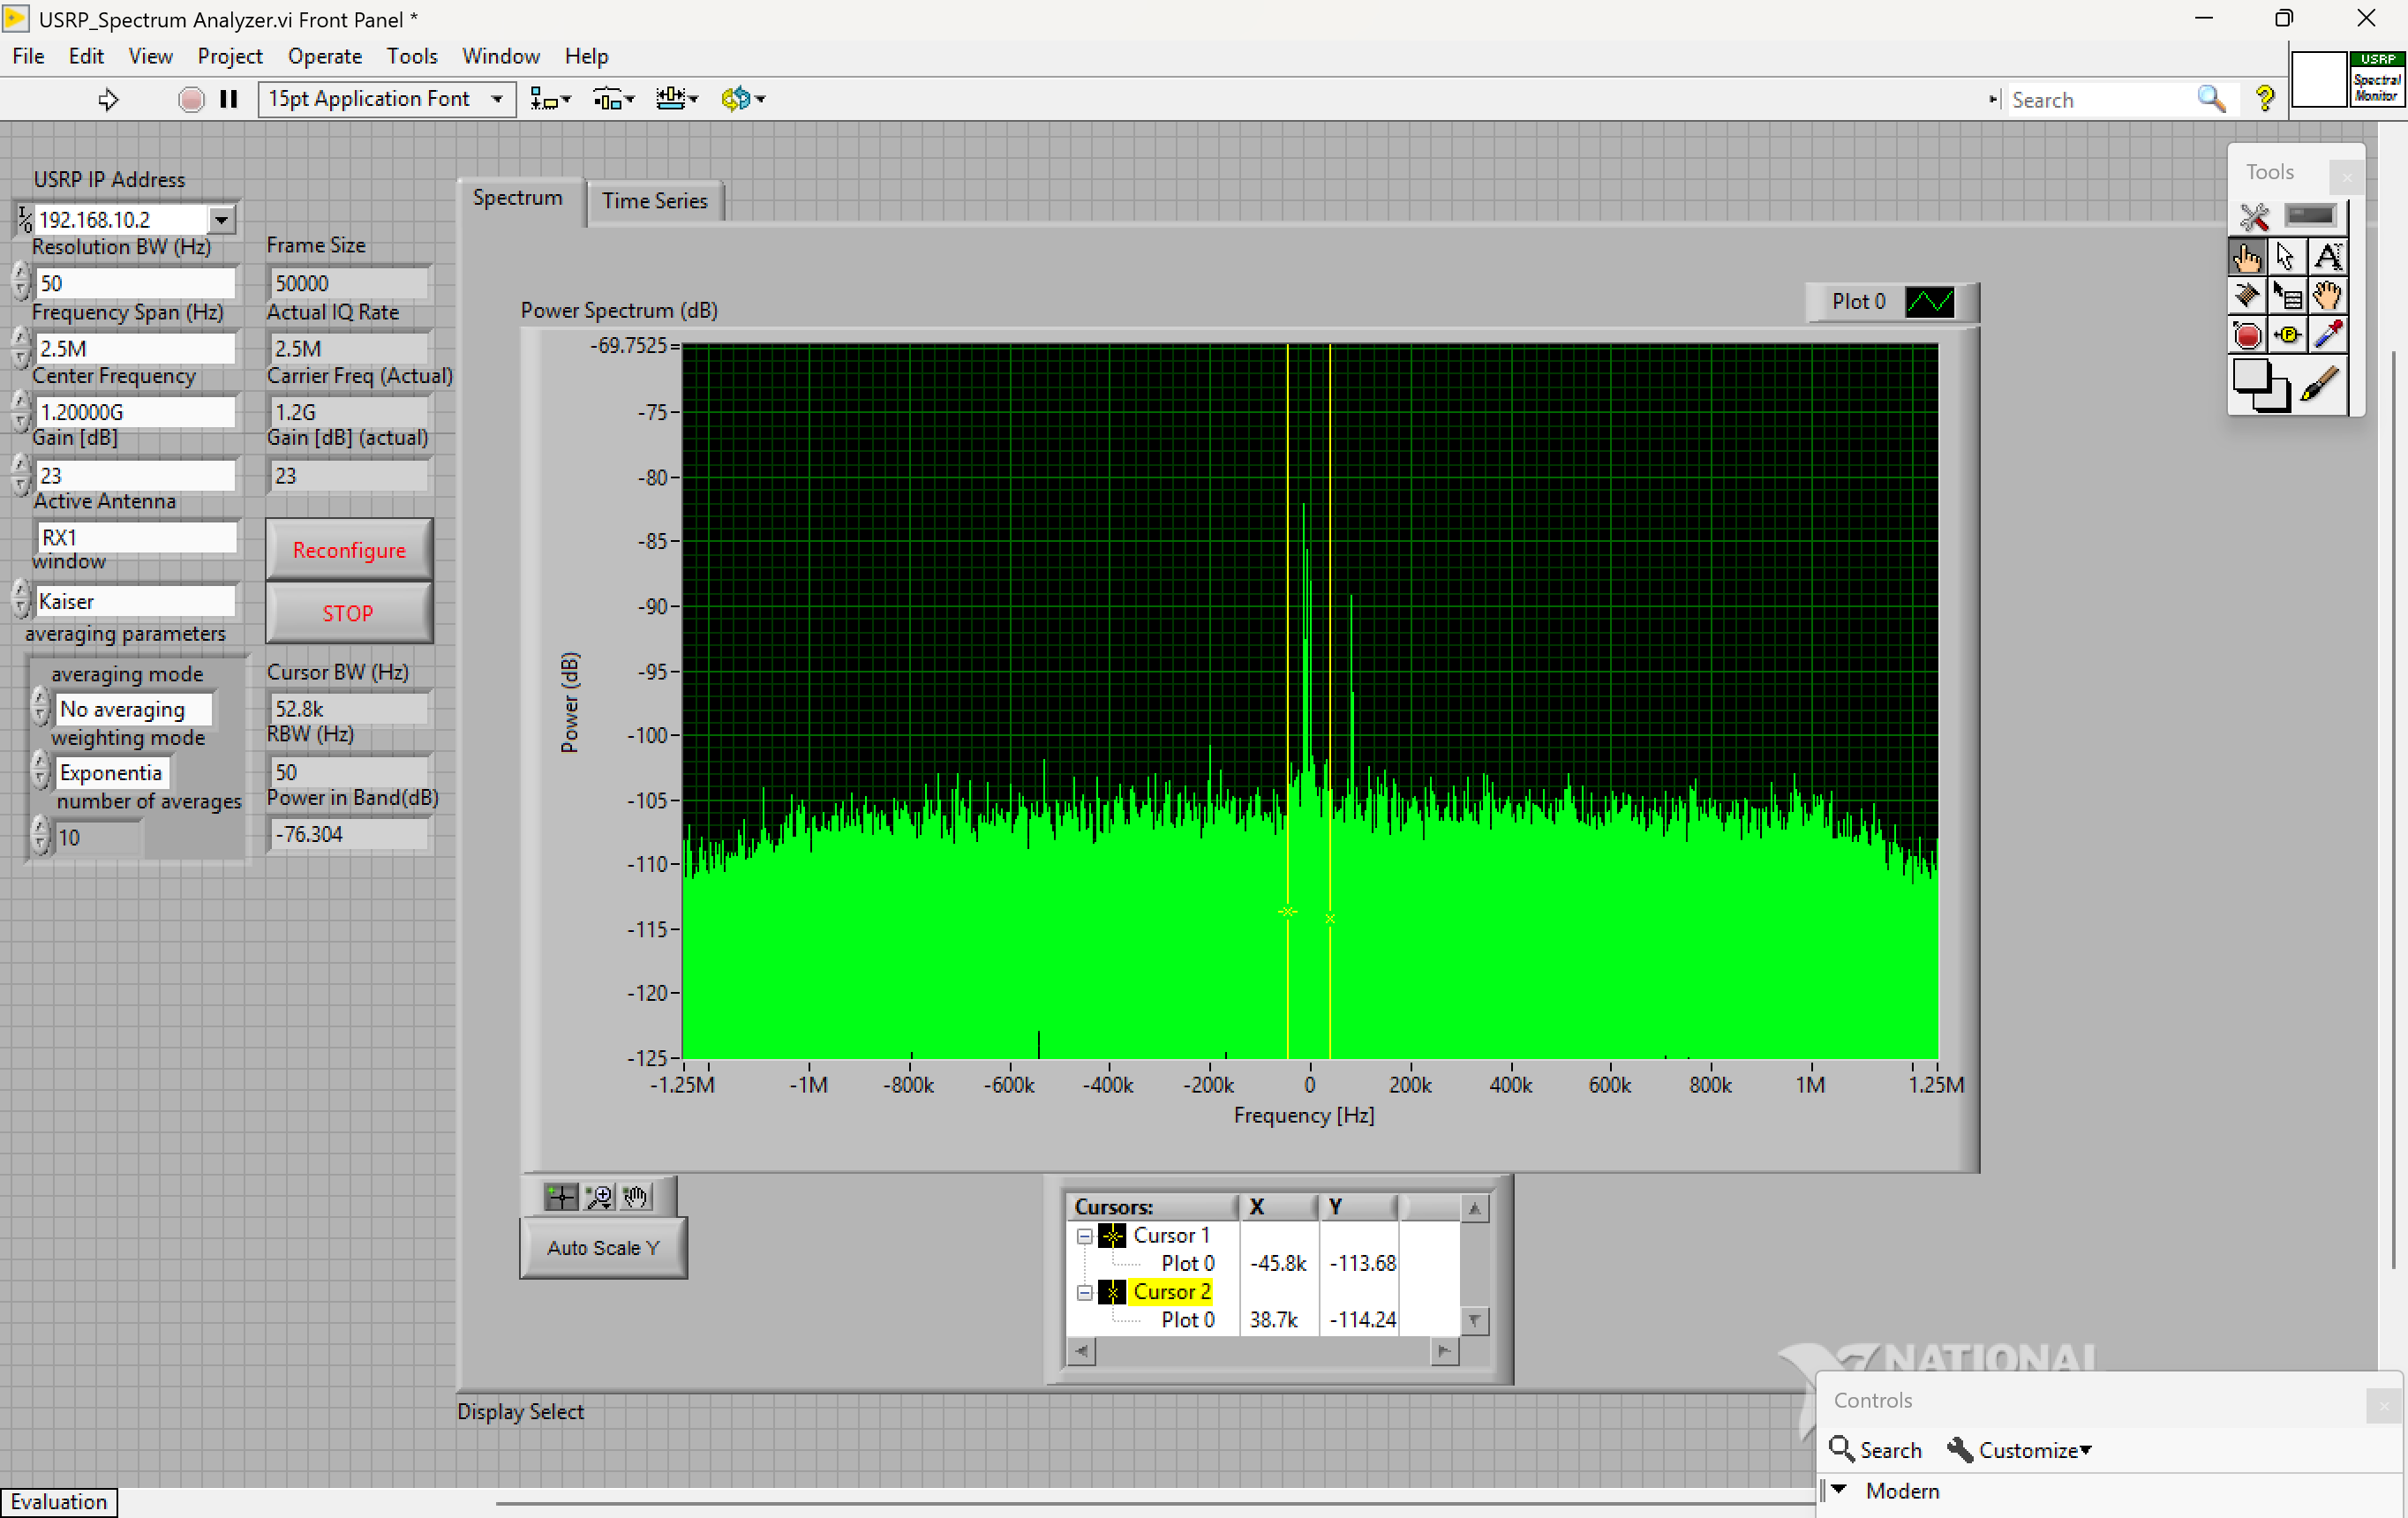
\includegraphics[width=0.7\textwidth]
   {../lab_ss/WES268B_Lab6_Part1-1-7_OFDM_measured-83khz_filter-parameter-0p5.png}
   \caption{1.1.7 - RX OFDM, $\beta = 0.5$}
\end{figure}
\par
\begin{figure}[H]
   \centering
   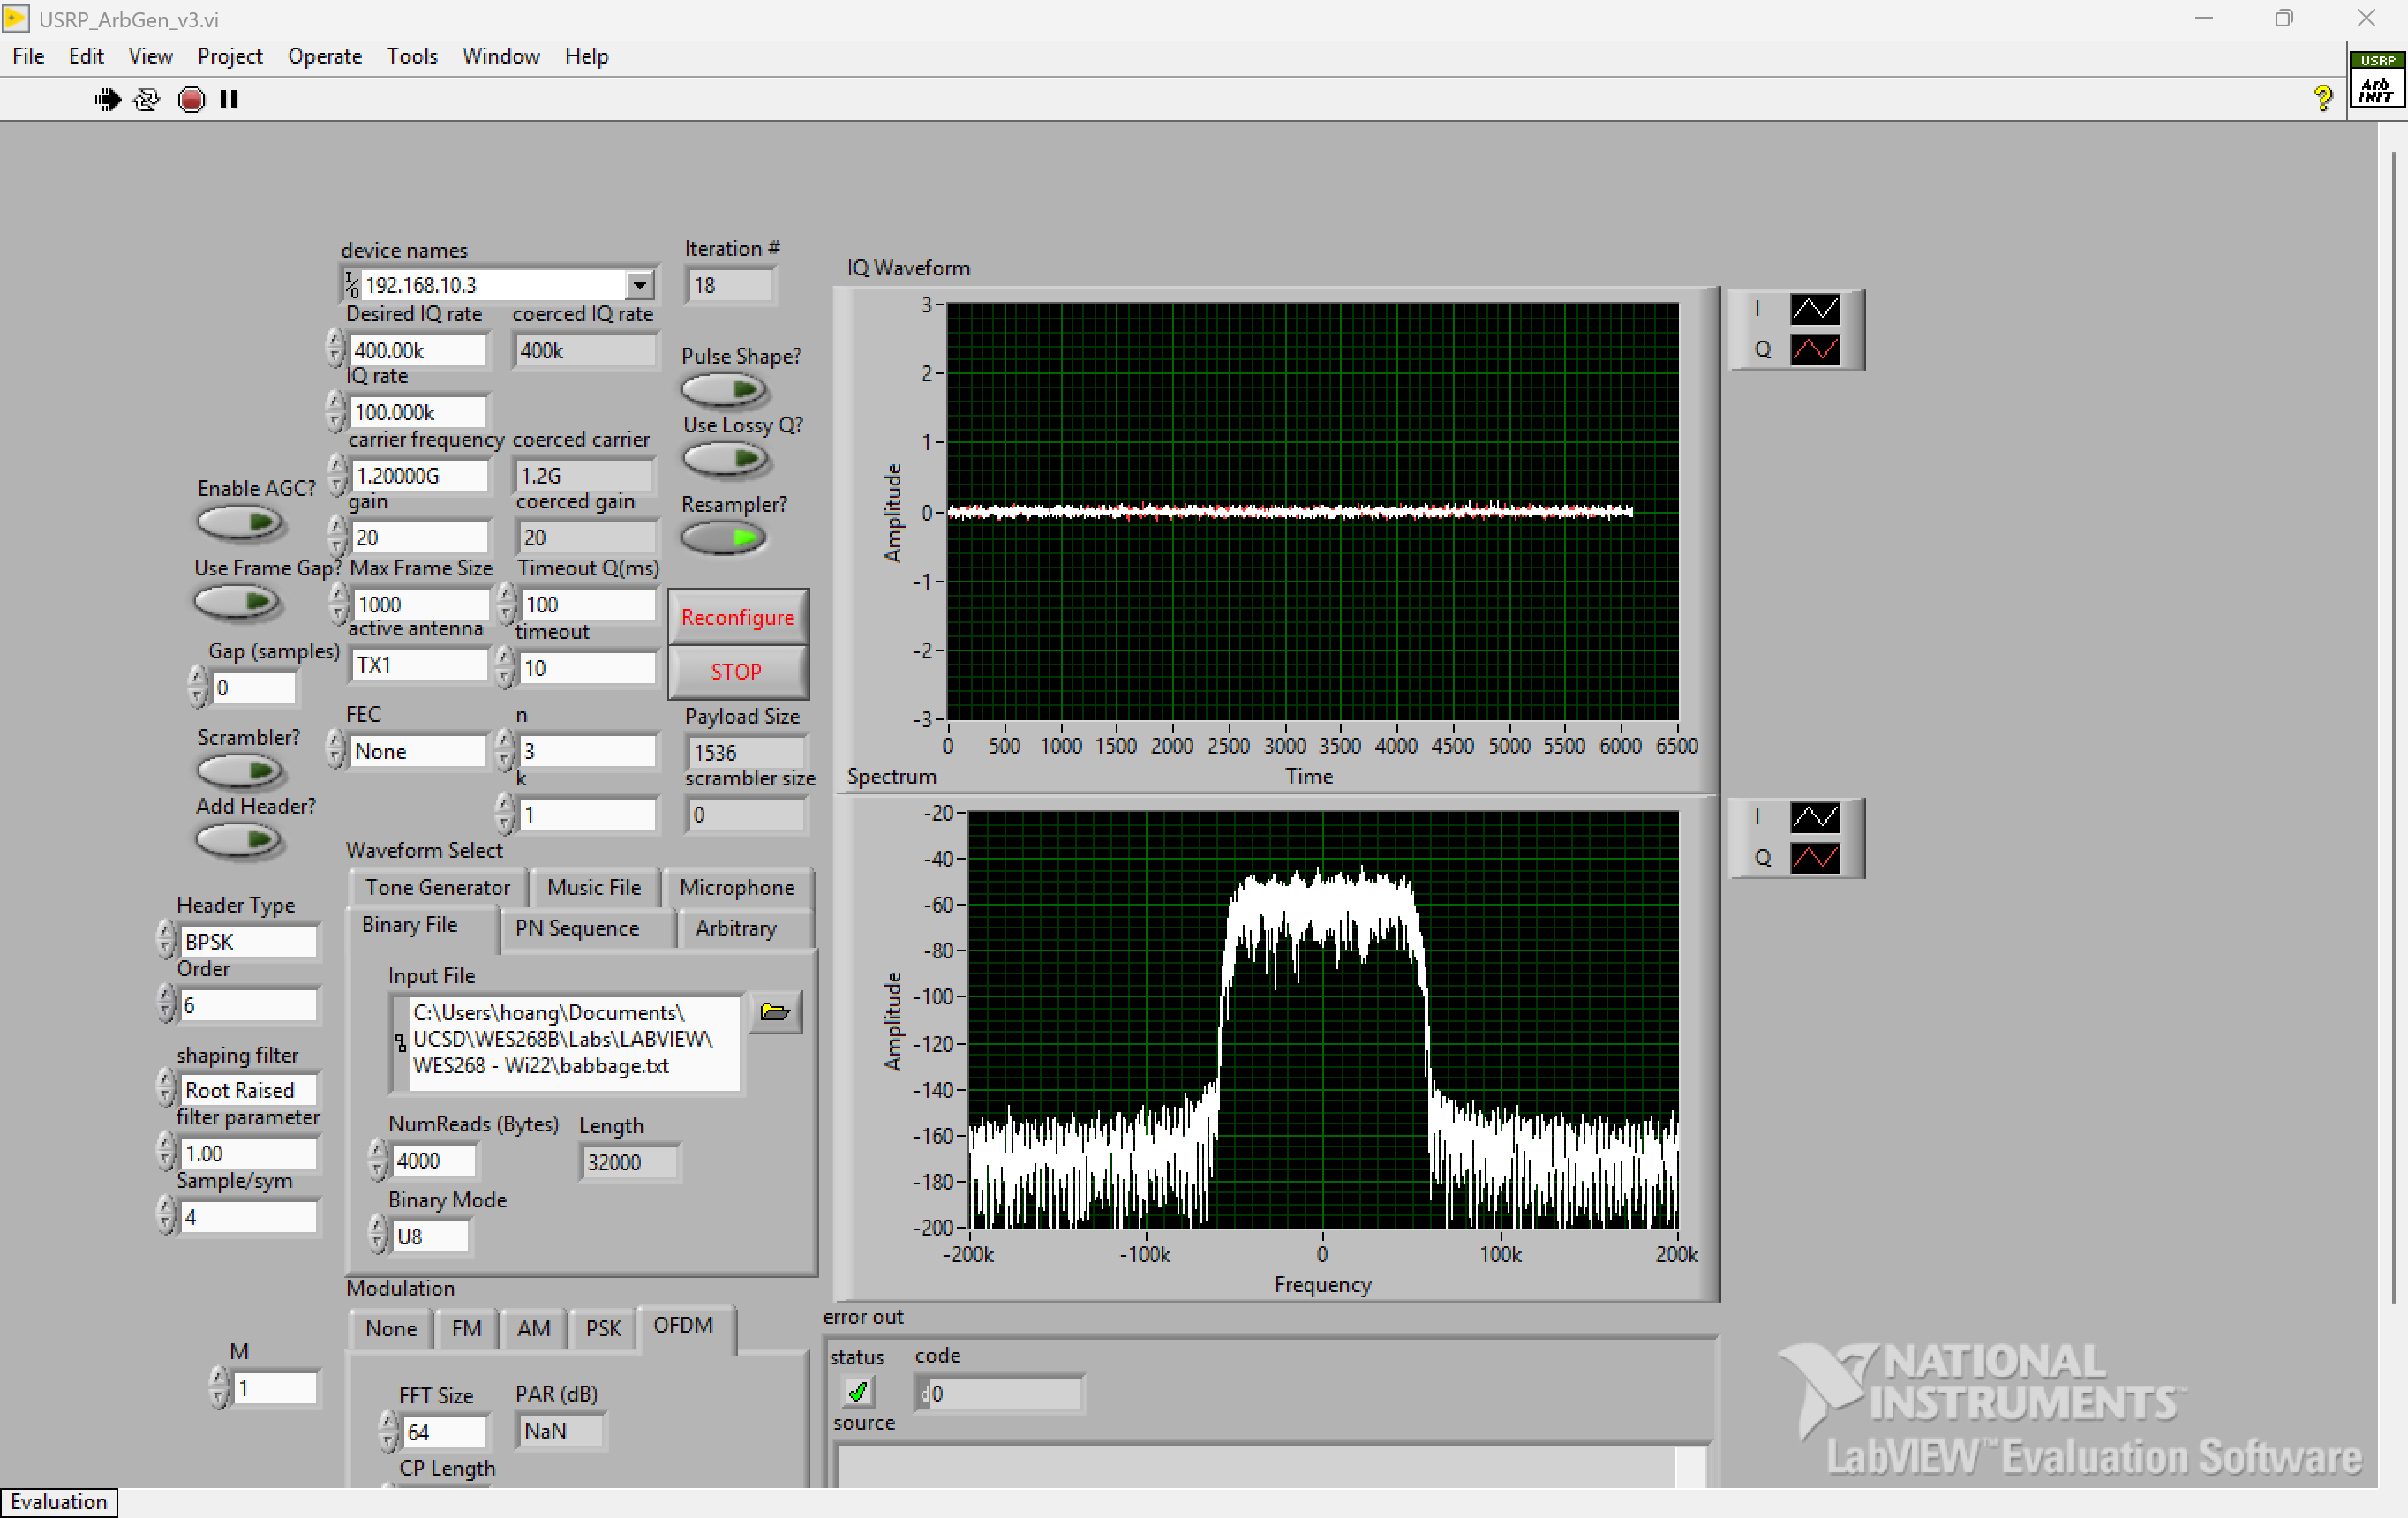
\includegraphics[width=0.7\textwidth]
   {../lab_ss/WES268B_Lab6_Part1-1-7_Tx_OFDM_filter-parameter-1.png}
   \caption{1.1.7 - TX OFDM, $\beta = 1$}
\end{figure}
\par
\begin{figure}[H]
   \centering
   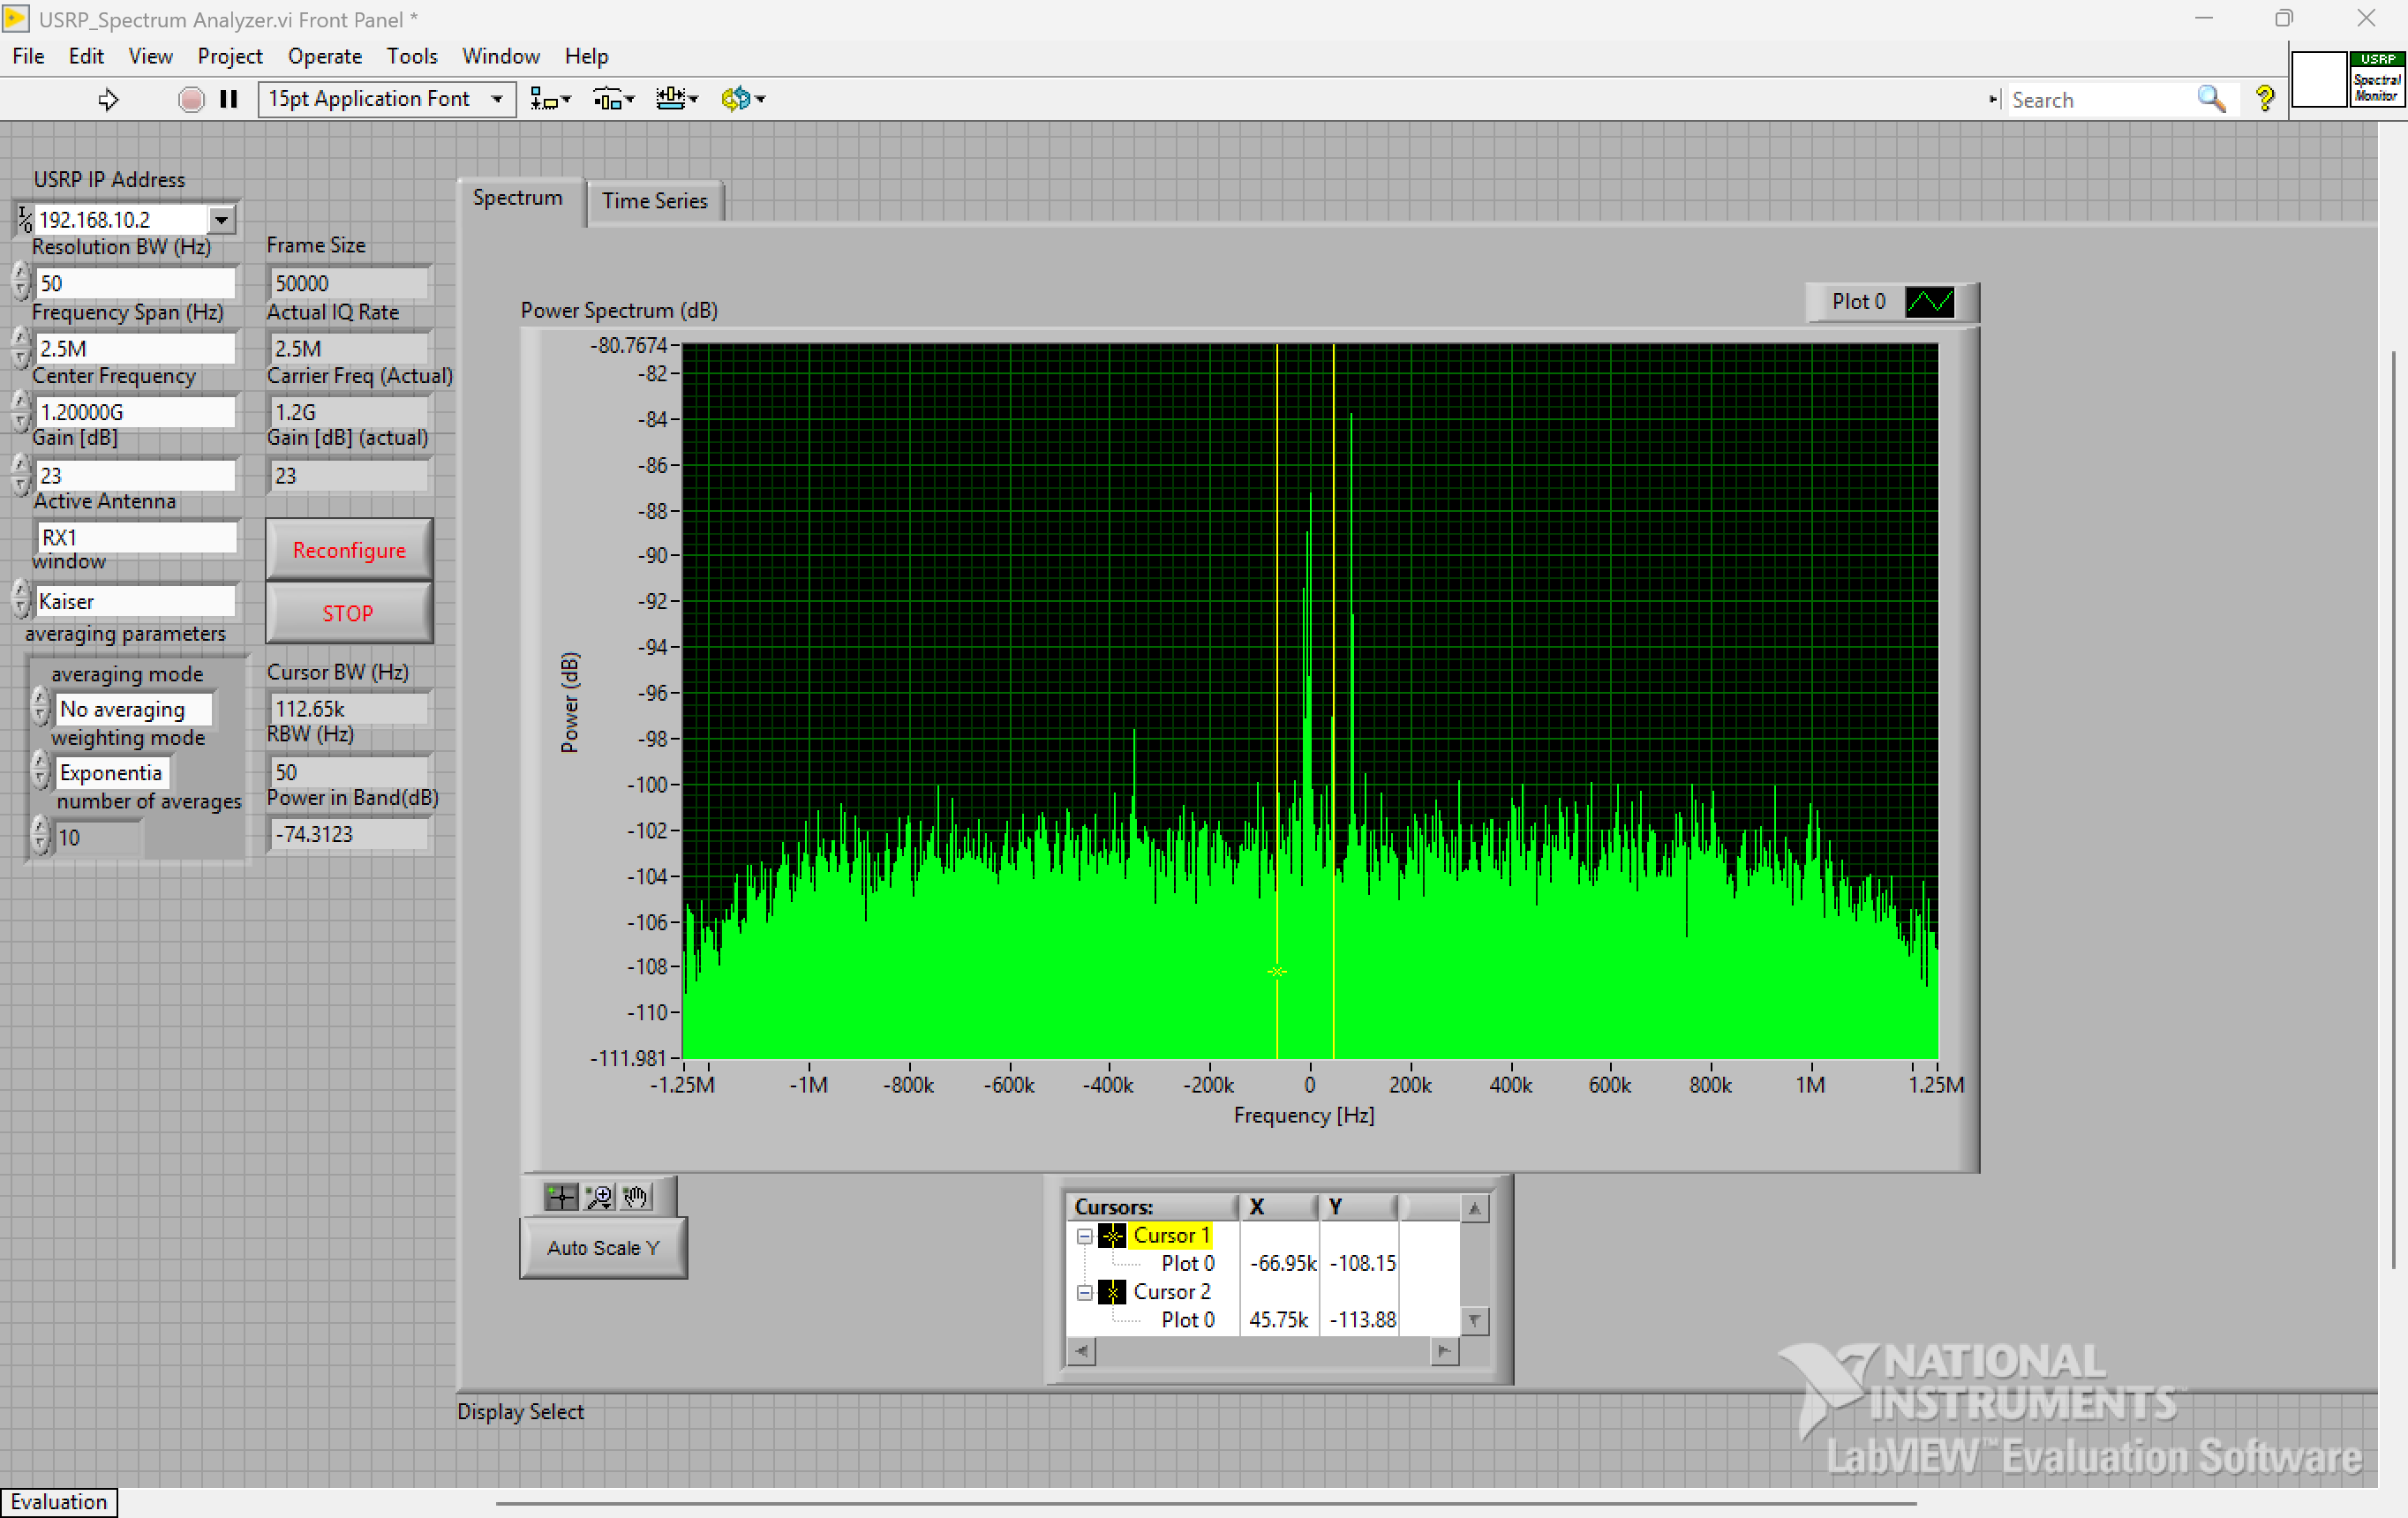
\includegraphics[width=0.7\textwidth]
   {../lab_ss/WES268B_Lab6_Part1-1-7_OFDM_measured-111khz_filter-parameter-1.png}
   \caption{1.1.7 - RX OFDM, $\beta = 1$}
\end{figure}
\par

\subsubsection{}
INSERT
\end{document}